\documentclass[12pt]{achemso}
\usepackage[utf8]{inputenc}
\usepackage{graphicx}
\usepackage{dcolumn}
\usepackage{bm}
\usepackage{amssymb,newtxtext,newtxmath,amsmath}
\usepackage{epsfig}
\usepackage{hyperref}
\usepackage{color, soul}
\usepackage{caption}
\usepackage{dirtree}

\renewcommand{\figurename}{Figure}
\renewcommand{\tablename}{Table}
\renewcommand\refname{References}
\renewcommand{\thefigure}{\arabic{figure}}
\renewcommand{\thetable}{\arabic{table}}

\newcommand{\bl}[1]{\textcolor{blue}{\textbf{#1}}}
\newcommand{\ml}[1]{\textcolor{magenta}{\textbf{#1}}}

\author{Fabian Weber}
\email{fweber13790@gmail.com}

\title[\texttt{achemso} demonstration]{\begin{minipage}{0.75in}
\includegraphics[width=0.75in]{./resources/00_Emblem.png}\end{minipage} ArchOnML - Documentation}

\begin{document}
\maketitle

\section{About}

ArchOnML (derived from "Archive-On-Machine-Learning") is a python package that allows setting up and conducting machine learning-assisted molecular design projects. It presents an interface between quantum chemistry packages (e.g. \texttt{gaussian}\cite{g16_cite} and \texttt{orca}\cite{orca_cite}) and machine learning packages that requires only minimal user input to start your own machine learning project.

\noindent It is designed to be useful to beginners in both machine learning and quantum chemistry, while offering the flexibility to implement new, user-defined descriptors or machine learning models specific to the project requirements.\\[-1.5em]

\noindent If you choose to use ArchOnML for one of your projects, please cite the program package source from the github. (https://github.com/archonml/archonml)

\noindent This documentation is split in three parts: The first part is a quick-start guide on what steps need to be done to use ArchOnML for your molecular design project. Here, we will just focus on how to set everything up to start as fast as possible. The second part is a users' guide with more detailed explanations on the possible options of the program package.

\noindent Finally, the third part is a developers' guide on how each individual module of the code is set up which is meant to help you extend the functionalities of ArchOnML to suit your specific project. To this end it will give pointers to what changes need to be made to add new descriptors, models or to incorporate further third-party quantum-chemistry program packages.

\subsection{Installing ArchOnML}

\subsubsection{Requirements}
ArchOnML requires the installation of additional python packages. It has been developed using python version 3.7, so we recommend using a similar version. It has been tested on UNIX and Windows machines, and should be running on Macintosh systems as well, when embedded properly. We highly recommend the use of an anaconda environment, since a fresh python installation is easier to build than add to an existing one, possibly producing version incompatibilities. After installation of anaconda, you can start configuring a new python 3.7 environment by running

\verb+ $ conda create -n AOML python=3.7 anaconda+

\noindent in a command prompt. After entering the newly created environment, the further required packages to install are\\[-2.5em]

\begin{itemize}
    \item numpy \\[-3.5em]
    \item pyquaternion \\[-3.5em]
    \item mendeleev \\[-3.5em]
    \item rdkit \\[-3.5em]
    \item sklearn \\[-3.5em]
    \item pickle \\[-3.5em]
    \item matplotlib\\[-3.5em]
    \item seaborn\\[-3.5em]
    \item numba\\[-3.5em]
    \item jupyter
\end{itemize}

\noindent all of which are freely available via the PyPI repositories (i.e. by installing them via the \verb+pip+ command) and/or anaconda. Some of these packages may require installation from a non-standard source, such as conda-forge or university hosted repositories. These can be specified, for example, by adding a \textbf{channel flag} (\verb+-c+) as in

\verb+ $ conda install -c conda-forge pyquaternion+.

\noindent You can find the channels by searching for the packages on the anaconda.org website. Finally, after installing all packages successfully, we recommend running

\verb+ $ conda update --all+

\noindent once, since some packages seemed to consistently produce errors, otherwise.

\noindent Lastly, ArchOnML comes with template IPython notebooks and python scripts that will help you set up a fresh project database in a step-by-step manner and monitor the learning process during ML training in an interactive way. Here, the notebooks serve as an interim graphical user interface - so we recommend installation and use of jupyter notebooks for executing the package. Prediction calculations, as well as learning curve generation are both designed to be done in larger-scale parallel fashion on a high-performance computing (hpc) cluster - and may thus be run in command-line, non-graphic fashion by executing further provided template python codes.

\subsubsection{Instructions}

ArchOnML does not require a special installation or set-up. You may clone the latest package version from github to your desired target location via

\verb+ $ git clone https://github.com/archonml/archonml.git+

\noindent Afterwards, to make the package accessible to your python environment, please add the path to the package (that is, the path to the folder \textbf{just above} the one that has the \verb+__init__.py+ file inside of it) to the \verb+$PYTHONPATH+ environment variable of your preferred command prompt (bash, zshell, etc.).

\noindent On windows machines, the \verb+$PYTHONPATH+ environment variable can be added through the system settings via

\noindent \verb+My Computer > Properties > Advanced System Settings > Environment Variables+

\noindent Note, that the exact route may look different on different versions of Windows (here, Windows 11).

\newpage

\subsection{Support}

If you have trouble with installing or using the program package, please contact the developers of ArchOnML directly via github's issues tab.

\texttt{https://github.com/archonml/archonml/issues}

\subsection{License Note}

ArchOnML is free software: you can redistribute it and/or modify it under the terms of the GNU Lesser General Public License as published by the Free Software Foundation, either version 3 of the License, or any later version.

\noindent This program is distributed in the hope that it will be useful, but WITHOUT ANY WARRANTY; without even the implied warranty of MERCHANTABILITY or FITNESS FOR A PARTICULAR PURPOSE.  See the GNU General Public License for more details.

\noindent You should have received a copy of the GNU Lesser General Public License along with ArchOnML. If not, see \verb+<http://www.gnu.org/licenses/>+.\\
Copyright (C) 2025, Fabian Weber.

\newpage
\section{ArchOnML Manual}

\subsection{1. Quick-Start guide}

\noindent ArchOnML comes with the option of screening both chemical and conformational space. Here, chemical space means that you wish to study chemical derivatives of a selected core structure by placing various user-specified chemical substituents at pre-selected sites. This may be useful when trying to optimize a chromophore's specific excitation wavelengths and/or its absorption strength. To conduct a standard chemical space screen, a user will need to follow these steps:

\begin{enumerate}
    \item Prepare the project folders and copy the template scripts.
    \item Prepare a \textbf{core structure}, whose derivatives shall be screened.
    \item Prepare a set of \textbf{substituents}, that shall span the chemical space.
    \item Run notebook ``01a'' for generating the database and third-party input files.
    \item Run the third-party quantum-chemistry calculations (i.e. (TD-)DFT, semi-empirical calculations, ...) and extract the target values (i.e. \textbf{label} values) for the training set.
    \item Run notebook ``02'' for training and saving the machine learning model for predicting a desired target value.
    \item Run the python script ``03'' for predictions on non-training data.
\end{enumerate}

\noindent A conformational screen, on the other hand, tries to predict the properties of the same molecule (complex) in different conformations. Screens of this type may be useful if you try to predict excited state properties in a vast amount of structural data, as obtained from molecular dynamics calculations. For this kind of screen, no substituents or core structure are needed. Instead, a file containing all conformations to study is used to set up the database by using notebook ``01b'' instead. 

\noindent In this quick-start guide, we will focus on how to set up a chemical space screen. Note that for all required files, there are templates available in the \bl{Sample\_GENERATOR} folder, so that you may use and modify them as desired. At the end, we briefly show the differences when setting up a conformational screen.

\subsubsection{Preparing the project folders}

\noindent To start a new project with ArchOnML, we recommend making a new folder for your project and placing another folder called \verb+GENERATOR+ in there. Into this folder, you should copy the contents of the \verb+Template_Scripts+ subfolder, contained within \bl{Sample\_GENERATOR} folder of the ArchOnML package. The resulting folder hierarchy of your new project may then look something like that (with folders highlighted in blue):\\[-0.7em]

\dirtree{%
.1 \bl{scratch}\DTcomment{the calculation space on your high-performance cluster}. 
.2 \bl{New\_Project}.
.3 \bl{GENERATOR}.
.4 \bl{Scripts}\DTcomment{a copied version of the \bl{Template\_Scripts}} folder. 
.5 01a\_Chemical\_Space\_DB.ipynb. 
.5 01b\_Conformation\_Space\_DB.ipynb. 
.5 02\_ML\_Module.ipynb. 
.5 03\_Predictor.py. 
}\vspace{1.0em}

\noindent Inside the \verb+GENERATOR+ folder, we now place two more required files for setting up the database of the chemical space screen. One of them is the core structure (with marked substituent positions), whose derivatives we wish to investigate and a library file pointing to substituent fragments that we would like to decorate the core structure with. It does not matter where you place these files exactly, or what they are named, since you must specify their path inside the \texttt{01a\_Chemical\_Space\_DB.ipynb} notebook, anyways. In the following, we briefly explain how these files are structured and what needs to be specified.

\newpage

\subsubsection{Preparing the core structrue}

\noindent ArchOnML is capable of producing all structural geometries automatically from a core structure and substituent structures. To ensure that these are generated correctly, however, the corresponding \texttt{.xyz} files need to be provided in a certain way. The core structure is the main molecule of interest that you want to modify by adding substituents. An example for the quinone template core structure is given below.

\begin{figure*}
  \centering
   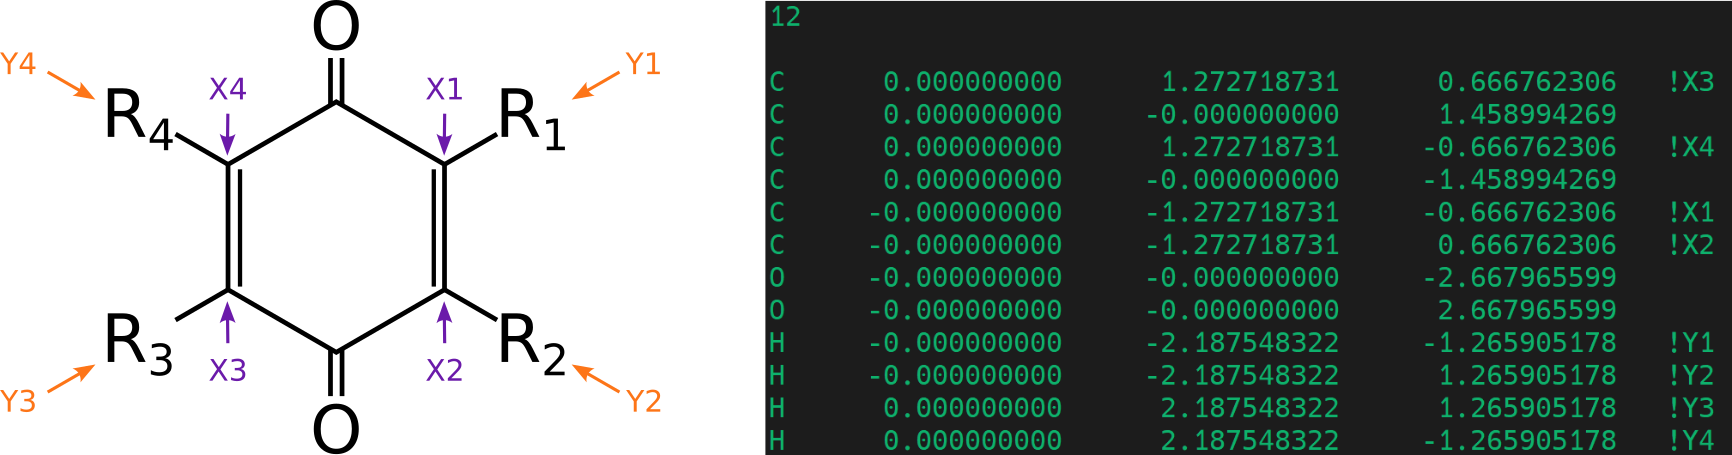
\includegraphics[width=16cm]{./resources/01_XYZ_Directionality.png}
  \caption{Example of a four-fold substituted quinone molecule as core structure. (left) Lewis structure with marked positions for the substituents. (right) Corresponding \texttt{CoreStructure.xyz} file with the planned substituent connectivities given as comments.}
  \label{FIG: 01_XYZ}
\end{figure*}

\noindent The \texttt{.xyz} file uses hydrogen atoms instead of ``R'', since otherwise you cannot display the structure in typical molecular viewers like \texttt{molden}. Instead, the tag ``R'' is captured by adding comments (marked with \textbf{!}) to specific atoms inside the \texttt{.xyz} file. Here, the direction of the ensuing substituent bond (\textbf{from core to substituent}) is encoded with letters - \textbf{from X to Y}. The numbering of substituents is captured by adding a numbering (starting with 1). Thus, the carbon and hydrogen atom that will form the C-R$\_1$ bond carry the comments \verb+!X1+ and \verb+Y1+, respectively. Finally, keep in mind that the numbering you provide in here will be \textbf{directly} reflected in the structure - which means that in the given example, position R$_1$ will become inversion symmetric to position R$_3$ and so on.

\noindent There is no limitation to the number of substituent sites - however, keep in mind that the size of the resulting database increases with $M^N$, where $M$ is the number of types of substituents and $N$ is the number of substituent sites. Also, the chosen substituents should only be modulating the behaviour of your core structure. For example, if you are studying excited state properties of a chromophore core and one of the substituents is a chromophore itself, it may become difficult to train a model on the effects that substituents have on the core structure as some excited states may end up centered on the substituents.

\noindent It is currently not supported to automatically connect mutliple substituents to the same atom, since that would require much more additional considerations about the resulting chirality. However, as a currently available workaround, you may merge several chemical sub-spaces together after generation. For such cases, please refer to the section of the users' guide on ``merging chemical spaces''.

\newpage

\subsubsection{Preparing the substituents}

\noindent The substituents are prepared in a similar fashion as the core structure, as they also require a directionality information - here with \textbf{X towards Y} translating to \textbf{from substituent fragment towards the core}. Note, that in the substituents only two atoms need to be marked, though. Therefore, the preparation of the substituents' files is slightly different (but overall faster) than for the core structure. We shall explain that on an example below.

\noindent Given that you want to place a -CH$_3$ substituent, you should first prepare an \texttt{.xyz} structure of (for example) CH$_4$. This structure may be optimized using (semi-empirical) structure optimization, so that all later optimizations are already closer to sensible structures. This CH$_4$ structure then needs to be saved with the name \verb+Opted.xyz+.

\noindent Next, you may open the \verb+Opted.xyz+ file with a molecular editing tool (e.g. \texttt{molden}) and replace the two atoms that will form the bond towards the core structure with \verb+XX+ and \verb+Y+ - which stand for a dummy atom and yttrium in molecular editing tools. This edited structure then needs to be saved to the file name ``Parent.xyz''. Similar to before, directionality follows the logic ``from X(X) to Y''. 

\noindent After preparing the (pre-)optimized substituent fragments, you only need to provide ArchOnML with a list of those substituents that you would like to use in your current project. Therefore, you need to supply a so-called \textbf{substituent library file} that contains names, IDs and an absolute path to the folder that contains the ``Opted.xyz'' and ``Parent.xyz'' files. The substituent library file is a normal text file that simply contains names, numeric IDs and addresses of the structures that you want to add to your core.

\noindent While this might seem overly complicated at first, this design choice makes it possible to just create a collection of substituent \texttt{.xyz} files once - and then re-use them for all future design projects by only adjusting the substituent library for your current project. An example library file then looks something like the following:\\[-1.2em]

\noindent \verb+Hydroxyl  1   /scratch/archonml/Sample_GENERATOR/Sample_Substituents/Hydroxyl/+\\[-0.3em]
\noindent \verb+Mehtyl    2   /scratch/archonml/Sample_GENERATOR/Sample_Substituents/Mehtyl/+\\[-1.0em]

\noindent Note that example templates are again available in the \bl{Sample\_GENERATOR} folder of the ArchOnML package for reference. Further, in case you want to add a single atom as a substituent (e.g. ``only -Cl''), just placing two atoms (e.g. ``H'' and ``Cl'') at \textit{any distance} will be sufficient for the ``Opted.xyz'' file. Then, just copy the file to ``Parent.xyz'' and replace ``Cl'' with ``XX'' and ``H'' with ``Y''.

\newpage

\subsubsection{Running notebook 01a\_Chemical\_Space\_DB.ipynb}

After both the substituent library and the core structure are set up, we can start to generate the infrastructure for the quantum-chemistry calculations and machine learning - i.e. the database. Let us assume for this example, that the current folder structure looks something like the following:\\[-0.7em]

\dirtree{%
.1 \bl{scratch}. 
.2 \bl{Substituents}. 
.3 \bl{Hydroxyl}. 
.4 Opted.xyz. 
.4 Parent.xyz.
.3 \bl{Methyl}. 
.4 Opted.xyz. 
.4 Parent.xyz. 
.3 .... 
.2 \bl{New\_Project}.
.3 \bl{GENERATOR}.
.4 CoreStructure.xyz. 
.4 Substituent.library. 
.4 \bl{Scripts}. 
.5 01a\_Chemical\_Space\_DB.ipynb. 
.5 01b\_Conformation\_Space\_DB.ipynb. 
.5 02\_ML\_Module.ipynb. 
.5 03\_Predictor.py. 
}\vspace{1.0em}

\noindent Here, the folder Substituents has all the substituents' \texttt{.xyz}-files and lies outside of the specific, new project. The files \verb+CoreStructure.xyz+ and \verb+Substituent.library+ contain the core structure and library of used substituents in this project, as described above. Now, we may start up one of the ``01'' IPython notebooks and go through the generation of the architecture step by step.\\[-1em]

\noindent The notebook serves as the multi-purpose generator tool for both setting up the database with respect to the substituted structures and folders, but also for generating input files for the third-party quantum-chemistry programs to obtain the raw data for training and predicting. It is divided into four sections that each come with a short explanation and many comment lines to explain the individual program blocks (often referred to as ``cells''). As a first time user, please pay close attention to the provided comments inside the notebook. Most pitfalls while using the notebook are likely explained somewhere.

\noindent Besides a general input section (that needs to be executed every time), the other sections deal with (A) selecting $N$ random molecules from the chemical space to generate a so-called \textbf{sample}, (B) generating the \texttt{.xyz} files of a selected sample and (C) setting up various third-party calculation inputs for a specific sample. Using this sample-oriented execution, the individual sections become independent from each other, such that you may restart the notebook and directly jump to section (C) to generate more/different quantum-chemistry calculations for a previously generated sample (e.g. first preparing the optimizations and later performing the TD-DFT).

\noindent Once you decided on a core structure and substituents, you may practically just follow along the instructions of each section to step-by-step generate your database and inputs. Note that in section (C) you will need to choose which third-party program you wish to use for your quantum chemistry calculations. To streamline the input inside ArchOnML to generate inputs for the different third-party quantum-chemistry programs, we decide to work here with pre-defined calculation types (e.g. "Opt" , "TDSn", ...) and calculation flavours (i.e. combinations of functional, basis set, etc.). For this purpose, you may want to consult the appendix of this documentation for the currently available standard calculation types - and / or the third-party program's own manuals. New types and flavors can be added by the user as well by adopting the provided format, as seen in the existing ones. An explanation to this can be found in the developers' guide.

\noindent Finally, in case your core structure features symmetry elements (mirror planes, inversion centers and such), you need to additionally avoid double counting of symmetry equivalent structures. How to do this is explained in more detail in the users' guide section on symmetry reduction and generator rulesets.

\newpage

\subsubsection{Running notebook 02\_ML\_Module.ipynb}

\noindent This notebook is aimed at training a kernel ridge regression (KRR) model for predicting a usually difficult-to-obtain or expensive-to-calculate quantity (the so-called \textbf{label} value) from readily accessible data (the so-called \textbf{descriptor} or \textbf{feature} values). For this purpose we need to have access to both labels and descriptors of a small set of reference molecules (the so-called \textbf{training set}) so that we can train the machine-learning model to relate descriptors to labels. After we are done with training, we can then use only descriptor data of unknown molecules (the so-called \textbf{prediction set}) to predict their label values.

\noindent When finishing your quantum-chemistry and semi-empirical calculations for the training set, you are able to start the training of the model. To do this, you need to specify in notebook ``02'' the name of a label (\texttt{LLabelL}) that you wish to train against - like (for example) \texttt{S1\_Energies}. Note, that at this point, ArchOnML will assume that there is a file called \texttt{S1\_Energies} inside the SEmpData folder that contains the obtained label values for your training set (which you should have ready at this point). The format of this file is in plain text with database IDs and label values in each line, like such:\\[-1.3em]

\noindent \verb+PROJ5       2.894277959+\\[-1em]
\noindent \verb+PROJ10      3.001237715+\\[-1em]
\noindent \verb+PROJ11      3.020668962+\\[-1em]
\noindent \verb+...+\\[-1.3em]

\noindent From our experience with the featured KRR model thus far, training sets for the ``standard model'' (implemented in the templates) should contain between 1.000 to 10.000 data points - and you should not attempt prediction spaces beyond 10.000.000. Beyond these, other models like neuronal networks will outperform kernel ridge regression - and these are still under development for ArchOnML.

\noindent To perform the training, the notebook \verb+02_ML_Module.ipynb+ may be run step-by-step as described in the comments of the notebook. In principle, ArchOnML will work with a list of objects (aptly named the MLOBJLIST inside the notebook), in which each entry represents one of the molecules of your database. In the beginning, ArchOnML will read in the raw data of the molecules, turn them into a native format (since the third-party codes might use different languages) and calculate descriptors from this raw data.

\noindent Since KRR predicts label values based on the similarity of known entries compared to an unknown ones, the notebook then produces distance matrices for all user-specified descriptors and then splits the training set into (active) training data and (hidden) testing data. Finally, the active training data is further split to perform a machine-learning technique called $K$-fold stratified cross-validation. This step is used to determine the best values of the so-called \textbf{hyperparamaters} of the model. More details on this can be found in the users' guide.

\noindent At each step of the cross-validation, ArchOnML will provide a map of the best combinations of hyperparameters. Finally, the ArchOnML wraps up all $K$ cross-validation steps, put together the optimized hyperparameters and predict the (so-far) hidden test data, to get an actual understanding of the model's performance. Note, however, that there are countless possible pitfalls on how to rate a machine-learning model (\textbf{overfitting} and \textbf{imbalanced datasets} to name a few) - thus we recommend to read more specialized literature on the matter.

\noindent A quick to understand example of a common pitfall is a scenario, in which all data has virtually the same label value. In this case, (seemingly!) accurate models may emerge with suspiciously low MAE's - but (most of the times) rather bad $R^2$ values. Here, it often turns out that the model has just ``learned to always guess the most common value'' and there is no actual "learned" connection between the descriptor and the label values.

\noindent Finally, you may save your model to hard disk, to later use it in predictions. Note that several program blocks of the notebook are supposed to be run only once during one session - so that you should rather restart the full notebook and go through it again step-by-step if you want to make some changes to how the learning proceeds - unless you know exactly which cells/objects you need to reset (which you learn eventually as you get more experienced with ArchOnML).

\newpage

\subsubsection{Running predictions with script 03\_Predictor.py}

\noindent After saving a model for you chemical space, you can start predicting the label values of all remaining structures. To do this, you first need to use the generator notebooks (\verb+01a+ or \verb+01b+) to generate and run the inputs for the ``fast, low-quality calculations'' for all remaining structures, such that you get all (semi-empirical) descriptors for all molecules. Note that this is a possibly very large amount of data and files. Hence, you should reduce the output as much as possible and throw away all unnecessary files on-the-fly during calculations on the hpc-cluster. For this purpose, we have prepared a few python scripts in the \bl{Analysis} subfolder of the program package, that can be executed within the job-scripts on your hpc-cluster.

\noindent The predictions are then performed by the \verb+03_Predictor.py+ script. This script reads in a previously saved, trained model as well as a sample library file that points to the locations of all the molecules that shall be predicted. Note, that by breaking down this library file into different smaller libraries, you can easily parallelize the prediction into batches. The parent library file (typically named ``SampleCalculations\_...'') is automatically generated by the \verb+01a+ or \verb+01b+ notebooks.

\noindent When deciding on the size of each prediction batch, we recommend to use a similar number of predictions as the size of your training set. The predictor script then writes an output file that, in each line, shows the ID-name of the predicted entry, its fingerprint and the predicted value.

\subsubsection{Preparing a learning curve with the LearnCurve\_Generator.py}

\noindent To see how well a property can be trained by an ML model, or identify possible problems in a dataset, it is advisable to create a learning curve. A learning curve is a graph that shows the performance of a machine-learning model when slowly increasing the amount of available training data. Here, ``performance'' is typically measured in terms of the mean absolute error, coefficient of determination $r^2$ or similar figures, when applying the model under consideration for predictions of \textbf{both} a fixed testing set and the currently used training set. In the following, the terms ``training curve/performance'' and ``testing curve/performance'' will thus relate to these two metrics.

\noindent To generate a learning curve with ArchOnML, one can thus make use of the LearnCurve\_Generator.py script provided in the \bl{Template\_Scripts} folder. This script will load the training data from a sample-calculations file, create the descriptors and the Kernel matrix and then perform the $K$-fold stratified cross-validation over and over for different active training data amounts (\verb+ActPerc+ option, see \verb+train_test_split+). It is thus, in principle, performing the exact same tasks as notebook ``02'' for many different settings of \verb+ActPerc+ - albeit in a non-graphic way, that is able to be run in parallel on an hpc system. If you are using this script, make sure that you have thoroughly optimized the grid settings for the CV procedure beforehand, though - which is easier to be performed in the interactive notebook. The trends in the performances and the gap between training and testing curves gives a lot of information about the diversity of the training and testing data or - from the reversed perspective - the generality of the trained model. Thus, there are a few behaviors to carefully analyze. In the following, a short primer on how to interpret learning curves and what behaviors to look out for is given. For more thorough understanding, please relate to more specialized literature.

\noindent Firstly, the overall performance needs to be evaluated. If the model is unable to predict the desired property from the descriptors for either training or testing data and does not improve significantly with more available data, it likely suffers from \textit{underfitting}. This means that the model itself is too simple to train the label property - which means that the descriptors in question need to be re-evaluated and adapted.

\noindent Secondly, one needs to consider the convergence behavior of the learning curves. Here, one typically observes that the testing performance becomes better with more available training data, while the training performance oftentimes gets worse with more available data. The reason for this can be interpreted as the model becoming better at generalization - which improves performance towards a set of data that it has never encountered before (i.e. the test set). The inverse is true for the training performance: In the beginning of a curve, when only very few data is available, the model usually performs really well, since there is almost no diversity in the set of molecules to consider. However, as more and more data gets added, the model loses its specialization towards these initial cases, since it now also has to accommodate for new entries that may not be similar to the initially available entries at all. Ultimately, both the curves thus converge towards some final quality - with either a large, small or no gap in between the performances. Note, that the training curve typically still always outperforms the testing curve - and can thus usually be understood as some sort of upper limit of the model performance. Considering the speed of convergence, it is obviously desirable that the model converges to a high performance rather quickly, because that means fewer training data is needed for a model to learn the relationship between descriptors and labels.

\noindent Thirdly, the gap between the performances needs to be taken into account. If the training curve always strongly outperforms the testing, this indicates a case of so-called \textit{overfitting}. In general, overfitting occurs when the trained model has become too specialized towards the training set and is thus unable to make predictions towards unknown cases. Note that this \textit{can} occur at any point during a learning curve - i.e. when the training and testing curves become strongly divergent at some percentage of available training data. Overfitting may indicate a too flexible model - i.e. the model has possibly too many training parameters that get highly specialized to the training set. This is somewhat countered by performing $K$-fold stratified cross-validation.

\noindent Finally, note that all of the above needs to be seen in the context of the underlying data itself. Since the test set should be selected at random from all available data, it might just so have happened that the particular set is more or less similar to the training data. Here, it is desirable, that the model is not showing large changes in performance for different training sets - a property that is referred to as \textit{robustness} of the model. To check for robustness, it is thus advisable to generate not only one, but several learning curves with different test sets each time and further compare the best and worst encountered model performances.

\subsubsection{Conformational space screening}

\noindent When studying the properties of molecules or molecular complexes, notebook ``01b'' can be used to set up the database and steer the further training behaviour. Note, that the training and predictions do not change on the front-end level of the code - such that you may just use the notebook ''02`` and the predictor ``03'' as usual. The only important thing to note is, that in the conformational space screen you are not required (nor supposed) to give a substituent library. In fact, by not specifying a library file (along another internal flag) the program package's behaviour changes in the required way to direct a conformational space screen.

\noindent It is important to understand, however, that the data used to train a model for conformational space screening must also fulfil the same uniqueness as for the symmetrically equivalent molecules of a chemical space scan. In other words: the training set should only contain unique conformations (without rotamers!) - such that no bias is present during training. After training, however, you may have as many copies of the same structure in your prediction set as you like. That means, that you should train the model on a set of unique structures - but that you can then predict the properties of all structures along any (for example molecular dynamics) trajectory of structrues, regardless of whether there are duplicates in this trajectory.

\noindent Therefore, we recommend using a program like \texttt{CREST}\cite{C9CP06869D} to first generate a set of unique conformations - and then use the trained model on whatever data you wish to screen.

\noindent Finally, since we are starting from (pre-)optimized structures already, no further optimization is required when generating the external program's inputs. In ArchOnML's ``language'' this means, that we would like to use the initial Guess in all calculations. For this purpose, there are specialized calculation types to be used that can be found in the appendix.

\newpage

\subsection{2. Users' Guide to ArchOnML}

\noindent The users' guide shall briefly introduce the options of the program package's individual steps and provide hints on how to approach more intricate problems such as merging different chemical spaces.

\subsubsection{Setting up the database}

\noindent In this section, noteworthy options of both versions of the ``01'' notebooks will be explained in the succession as they appear in the notebooks. Additionally, the purposes of the most important objects and lists of the database are explained in layman's terms. For in-depth details, please refer to the developer's guide instead. Note, that the data type of the objects and parameters is highlighted when useful.

\paragraph{GenInstance} - This \texttt{object instance} is the generator of calculations and folders. It contains methods to initialize all folders and structures, as well as writing the input files of the desired quantum-chemistry package. It depends on the core-structure and substituent library file, as well as the planned folder structure given by the remaining parameters. Detailed descriptions of its structure will be given in the developer's guide.

\paragraph{FINGERPRINTS} - This \texttt{list-of-lists} contains identifiers for each of your possible structures. The length of the list directly reflects the maximum amount of possible structures to generate from your specified core structure and substituent library - or the number of conformers contained inside the provided the conformations file, in case you are performing a conformational space screen. Note that this list is generated by \texttt{GenInstance} \textbf{without} symmetry considerations - and should thus be shortened by the user after generation, if necessary. Also the fingerprints of a conformational screen will behave differently than the ones of a chemical space screen.

\noindent For the chemical space screen, each individual entry of the list will directly encode the chemical composition of the core structure and substituents provided inside the substituent library file. For example, assume that the substituent library contains four entries with the names (and IDs) Hydrogen (1), Methyl (2), Cynano (3) and Ethyl (4). If the core structure then features four substituent positions ($R_1$ to $R_4$), then a fingerprint [1, 2, 2, 3] will refer to a chemical derivative that has been substituted with hydrogen at $R_1$, methyl on positions $R_2$ and $R_3$ and a cyano-group on position $R_4$.

\noindent For a conformational scan, the FINGERPRINT will be a \texttt{list-of-lists} in which the individual entries have always length 3. Here, the first and second entries of the individual fingerprint serve simply as a pointer for ArchOnML to sort the data belonging to the individual structure inside the correct folders. The third entry, however, encodes which exact structure it stems from inside the provided conformations file (i.e. \texttt{ConformerStrucFID} inside the ``01b'' notebook).

\paragraph{On symmetry} - Note, that depending on the symmetry situation of the core structure and how the $R$ were assigned in the core structure \texttt{.xyz} file, the fingerprint [3, 2, 2, 1] might be a symmetry-equivalent duplicate of [1, 2, 2, 3]. Such duplicates need to be avoided or removed, since otherwise the machine learning will become biased later on, as not all possible structures are equally likely represented. For a simple case like the quinone example, a ``brute-force'' method of removing the duplicates is shown in the template notebook. Here, we define a set of boolean conditions that are evaluated for every possible fingerprint, to decide whether the current fingerprint is a unique one - or whether we have encountered its symmetry equivalent before. Note, that you may also deliberately remove specific fingerprints this way. For example, you might want to add a specific substituent only once or twice at maximum inside any given fingerprint. Here, you could add a new boolean to check how many of the desired substituents have been counted inside the same fingerprint.

\noindent For larger or more complicated cases, we recommend rather generating an already symmetry-reduced list of fingerprints right away instead of removing the duplicates from the automatically generated list step-by-step, since the brute-force process shown in the template for quinone can become very time-consuming. One way to achieve this, is to (for example) pre-generate ``halves'' of the fingerprints and then put them together in a way that avoids duplicates by design. Here is an example of what that approach would mean:\\

\noindent Suppose that there is a mirror plane inside the core structure and there are 4 possible substituent positions, where the positions $R_1$ and $R_4$ as well as $R_2$ and $R_3$ can become pairwise mirror-images. In such a scenario, a fingerprint [1, 2, 3, 4] will be symmetry equivalent to [4, 3, 2, 1]. Then, we generate the list of all "halves" of fingerprints - that is, a list containing entries like [1, 1],\linebreak \phantom{} [1, 2], [1, 3], ..., [2, 1], [2, 2], ..., and so forth. We can then produce the (already symmetry-reduced) list of full fingerprints from the halves by using code like:\\[-1.5em]

\verb+for ii in range(len(Halves)):+\\
\verb+    for jj in range(ii, len(Halves)):+\\
\verb-        FINGERPRINT.append(Halves[ii] + Halves[jj])-\\[-1.5em]

\noindent Here, the idea is to only generate the ``upper half'' of the triangle of all possibilities (including the diagonal), by having \texttt{jj} run over all halves starting from the current \texttt{ii}, however. Make sure, that after generating the fingerprints by yourself this way, you need to \textbf{overwrite} the existing FINGERPRINTS placeholder inside the \texttt{GenInstance} object and the notebook main instance. You can achieve this by using\\[1.0em]

\verb|GenInstance.FINGERPRINTS = dc(YourList)|\\

\phantom{}\\[-10.0em]

\verb|FINGERPRINTS = dc(YourList)|\\[1em]

\noindent Other symmetry operations may be achieved in a similar fashion - but an automatic scheme is highly desirable for the future.

\paragraph{StrucLib file} - This file contains all possible structures' internal identifiers, fingerprints and the path to its generated \texttt{.xyz} file. Note that this list is generated from the \texttt{FINGERPRINTS} - and thus needs to be generated (only once) \textbf{after} reducing the number of entries by symmetry considerations and/or additional generator rules as explqained above. The internal identifiers are constructed from your given project name \texttt{ProjName} plus an integer, e.g. \texttt{PROJ126}. These IDs will also serve as folder names in which the calculations of the quantum chemistry packages will be performed. In case you want to look up an entry of the database with respect to a specific fingerprint, you may thus search this file for the exact fingerprint that you are interested in.

\noindent Note, that not all guess-structure files are generated immediately, as this would require a large amount of time and disk space before you had the chance to train on any set of molecules and see, whether machine-learning can be applied to your problem at all. Instead, the generator works in batches of \texttt{N} sampled molecules at a time, which is controlled by the \texttt{GenInstance.sample(...)} method, described below.

\paragraph{Fold\_L1 and Fold\_L2} - These two \texttt{integer} parameters of the database will control the folder structure of the database. In general, input-output operations become slow when more files and folders are in one place. If there are several thousands of files present in a folder, this look-up process for a specific named file becomes slower and slower. Thus, using the parameters \texttt{Fold\_L1} and \texttt{Fold\_L2}, the data is distributed into folders and sub-folders of data, such that each individual one will have less files inside. To ensure that the user can still navigate the database by hand (if necessary), we decided arbitrarily that there are two levels of such branches.

\noindent In the case of a chemical space screen the folder numbering directly corresponds to the fingerprints. Assuming \texttt{Fold\_L1} and \texttt{Fold\_L2} were chosen as 1 and 2, respectively, then the calculations belonging to [1, 2, 2, 3] would be found somewhere inside the database as \bl{../../DATABASE/1/1\_2/}. Our recommendation is to leave \texttt{Fold\_L1} as 1 and change \texttt{Fold\_L2} according to about half the length of the overall fingerprint.

\noindent For a conformational screen, the folder structure changes to a "plain rectangular shape" depending on the values of \texttt{Fold\_L1} and \texttt{Fold\_L2}. That means, that the first layer of folders ranges from 1 to \texttt{Fold\_L1} and the second ranges from 1 to \texttt{Fold\_L2}. Before actually creating the folder structure (when calling \texttt{gen\_db\_folders}), the notebook will inform the user about how many structures will end up in each lowest-level folder with the current setting. As a rule of thumb, you should try to avoid going beyond an order of $10^3$ of structures in one folder.

\paragraph{GenInstance.sample(...)} - This method of the generator module will pick a user-defined amount of random fingerprints and bundle them together into one sample. Note that the option \texttt{FixedSeed} will activate or deactivate a fixed seeding for the randomness. Also, take note that even fixed seeding will behave differently on different physical computers, as the artificial randomness is still hardware-dependent. In other words, a fixed seed will always produce the same randomness, as long as it is executed on the same computer. The \texttt{sample} method will keep both a local record of the current sample (\texttt{LocSetLib}) as well as a permanent record of which fingerprints have been bundled in any previous sample (\texttt{SampLib}). Thus, make sure not to overwrite the local sample's \texttt{LocSetLib} file by changing its name each time. This way, you can stepwise increase your database in batches - while avoiding double counting the same fingerprints.

\noindent In case you want to have specific fingerprints included inside a sample, you may use the \texttt{StrucLib} file (which contains all possible IDs and their fingerprints) and add them by hand to an existing \texttt{LocSetLib} file. Note, though, that a purely data-driven model should only be trained from fully randomized sampling as everything else will introduce \textbf{human bias}... Also, please do not forget to add the specific entries to the \texttt{SampLib} file as well, in this case.

\paragraph{Part B Cells} - These program blocks will generate the \texttt{.xyz} files of the currently selected local sample by calling the generator method \texttt{full\_junc\_once} in parallel. There are no real options to this part, so these program cells of the notebook can be used as-is.

\paragraph{GenInstance.gen\_calcs(...)} - This method of the generator module writes the actual input files of the specified QC program package (\texttt{QCPack}) - currently \texttt{orca} or \texttt{g16}) for the desired calculation type (\texttt{CalType}) and calculation flavours (\texttt{CalFlav}). The method will also produce a new sample calculation file (\texttt{CalPathLib}) which will contain the paths to all calculations of the current sample for convenient usage in hpc job-scripts and automated analysis. A list of possible calculation types and flavours is given in the appendix. Note that not all types and flavours can be defined for all programs, as not all basis sets and such are available across all QC packages. New types and flavours can be defined by the user by copying and adjusting the provided existing ones. Also, in case you want to set up ArchOnML with a new quantum chemistry package, you should stick to the general workflow of the existing generators, so that the overall process stays streamlined.

\noindent Note that some types of calculations will require previous calculations to be performed in between running the generator steps. For example, you should only use a fully optimized structure for a TD-DFT calculation of excited states and likewise, an optimization should be started from a previously pre-optimized structure. Also, some of the calculation types allow for additional keyword arguments like \texttt{nstates} as the number of states considered in a TD-DFT calculation.

\subsubsection{Options and important (object) instances while running the training}

\paragraph{General Definitions} - In the beginning of notebook ``02'', you first need to specify which third-party quantum-chemistry program was used in the calculations (\texttt{LQCPack}) and what quality of theory was used for generating the raw data for the descriptors (\texttt{LQC\_low}) and the target (label) values (\texttt{LQC\_high}). In the list \texttt{LLabelL}, you then need to add the names of the labels you want to train on. Note that input must be given in quotation marks (i.e. \texttt{string} data type). Also, for each label value that you specify, ArchOnML will look for a file with the \textbf{same name} inside the \texttt{MergePath} you specified in notebook ``01'' (by default the folder is called ``SemiEmpData\_ProjectName''). From this file, it will read the label value of the training set. The list \texttt{LDataL} defines which raw data shall be read from the outputs of the quantum chemistry calculations. In case you need to generate new raw data for new descriptors, these can be added as new arguments to \texttt{LDataL}.

\noindent The next two options will define how the descriptors will be generated from the raw data. The \texttt{MOWin} parameter controls how many orbitals will be used for all descriptors that include multiple orbitals. Note that this window is defined as additional orbitals around the HOMO-LUMO-gap. The default value of 4 will therefore include the orbitals HOMO-4, ..., HOMO-0, LUMO+0, ..., LUMO+4. Finally, the \texttt{LDescL} gives the \texttt{list} of descriptor names (in \texttt{string} format) that shall be generated by the descriptor \texttt{object instance} called \texttt{DescInst}. A list with all currently available descriptors can be found in the appendix.

\paragraph{MLOBJLIST} - This \texttt{list of object instances} is the central container for all database entries - both during training and prediction. The list contains several \texttt{MLEntry} objects, each of which is initialized with the \textbf{meta-data} defined in the general definitons - i.e. what program was used, which raw-data and descriptors should be created for this object and such. Its main purpose is to carry entry-specific information and interact with the other object classes defined in ArchOnML. Note that the \texttt{MOWin} is in fact a global parameter for the \texttt{MLEntry} class. For more information on the class objects of ArchOnML, please refer to the developers' guide.

\noindent Inside the notebook, you may use the ``SampleCalcs'' files (which were created during generation of the calculation inputs in notebook ``01'' - see the file name specified in \texttt{CalPathLib}) to conveniently add the sampled molecules to the \texttt{MLOBJLIST}. If you performed several samples, just keep adding more files in the same way by copying the program cell of the notebook and changing the filename accordingly.

\paragraph{Merging of raw data; ArchOnML's native format} - To make it possible that the training can proceed smoothly for any given external quantum chemistry package, ArchOnML reads in the raw data from the output files of the third party package and translates it into its own native format (so-called \textit{parsing} of data). This merging process also facilitates the training on a technical level, since after merging the raw data (needed only once per database entry!), all the data for a single entry is in one compact place, instead of possibly several long output files. The merged files will be written into the \texttt{MergePath} you specified during database generation (notebook ``01''). It follows the same sub-folder hierarchy of  

\noindent In case you want to set up ArchOnML with a new quantum chemsitry package, it will be necessary to write a \textit{parser} accordingly, such that the native file format can be obtained. For pointers on how to achieve this, please refer to the developers' guide.

\paragraph{Data management with DataInst} - This \texttt{object instance} of the so-called \textit{DataTens class} (short for data tensor) is the object that organizes the descriptor data for the kernel ridge regression (KRR) specific training and prediction. It is able to split the training data into test and training sets and set up the data for a stratified \textit{K}-fold cross-validation with varying amounts of ``active'' training data, to obtain learning curves for your model. To understand what this means, we briefly explain how the kernel ridge regression model performs training and predictions.

\noindent In kernel ridge regression, the target value $E^\mathrm{pred}$ of an unknown entry $M'$ is related to the similarity function $f(M', M_i)$ of the unknown entry towards each training set entry $M_i$ times its respective trained weighting factor $\alpha_i$. The $M_i$ form a static set of references $\mathbf{M}$ (i.e. the training set).\\[-3em]

\begin{equation}
    E^\mathrm{pred}(M', \mathbf{M}) = \sum\limits_{i} \alpha_i f(M', M_i)
\end{equation}

\noindent In other words, if an unknown molecule is very similar to one (or several ones) inside the training reference, the model might assume that it's predicted property should also be more similar to these entries. For quantifying similarity, abstract \textit{distances} $d_g (M', M_i)$ between molecules need to be calculated. For each descriptor $g$, it is thus necessary to calculate a distance matrix between the reference set and all unknown molecules that shall be predicted. This is one of the tasks that is automatically carried out by the \texttt{DataInst} object.

\noindent Besides the weighting coefficients $\alpha$ that are optimized during training, the KRR model has two more parameters $\lambda$ and $\sigma$ that affect the model's performance. They enter the model during the optimization of the $\alpha$ in the equations and how the similarity function is defined:

\begin{equation}
    \min \phantom{}_\alpha \sum\limits_{j} \big( E^\mathrm{pred}(M_j, \mathbf{M}) - E_j^\mathrm{label} \big)^2 + \lambda \sum\limits_{j} \alpha_j^2
\end{equation}

\begin{equation}
    f(M_i, M_j) = \exp \Bigg(-\Bigg( \sum\limits_{g} \frac{d_g(M_i, M_j)^2}{2 \sigma_g^2}\Bigg)\Bigg)
\end{equation}

\noindent The meaning of $\lambda$ and $\sigma$ can be roughly summarized as measures to counteract noise in the data ($\lambda$) and the strictness with which to compare entries ($\sigma$). The latter can be understood directly, as the similarity function $f(M_i, M_j)$ is practically a sum over gaussians with respect to each distance between two molecules $d_g(M_i, M_j)$ for a descriptor $g$, where $\sigma_g$ is a measure for the width of the specific gaussian. As $\sigma_g$ becomes very large, the similarity evaluation becomes less and less strict, as the exponential's argument goes towards zero more easily.

\noindent Note that each descriptor $g$ has its own $\sigma_g$ associated to it - leading to $N$ individual parameters plus the one for $\lambda$. Unfortunately, these $N+1$ parameters are not optimized by training the model - and thus need to be optimized outside of training. Such parameters are referred to as \textit{hyperparameters} in machine-learning. Therefore, to fully optimize these hyperparameters on a grid with \texttt{CVGridPts} for each parameter, a number of \texttt{CVGridPts}$^{N+1}$ individual models would need to be trained and evaluated for their performance. To speed up this optimization process, three different optimizers are currently available in ArchOnML. The details on these will be given further below. 

\noindent Further, to avoid overfitting when choosing hyperparameters, ArchOnML can perform a technique called stratified $K$-fold cross-validation. Here, the training data is further broken into $K$ smaller parts that will be optimized in separate blocks where the final  hyperparameters are averaged from all $K$ individual optimizations. Below is a visual representation of how the data is organized - and how the training works.

\begin{figure*}
  \centering
   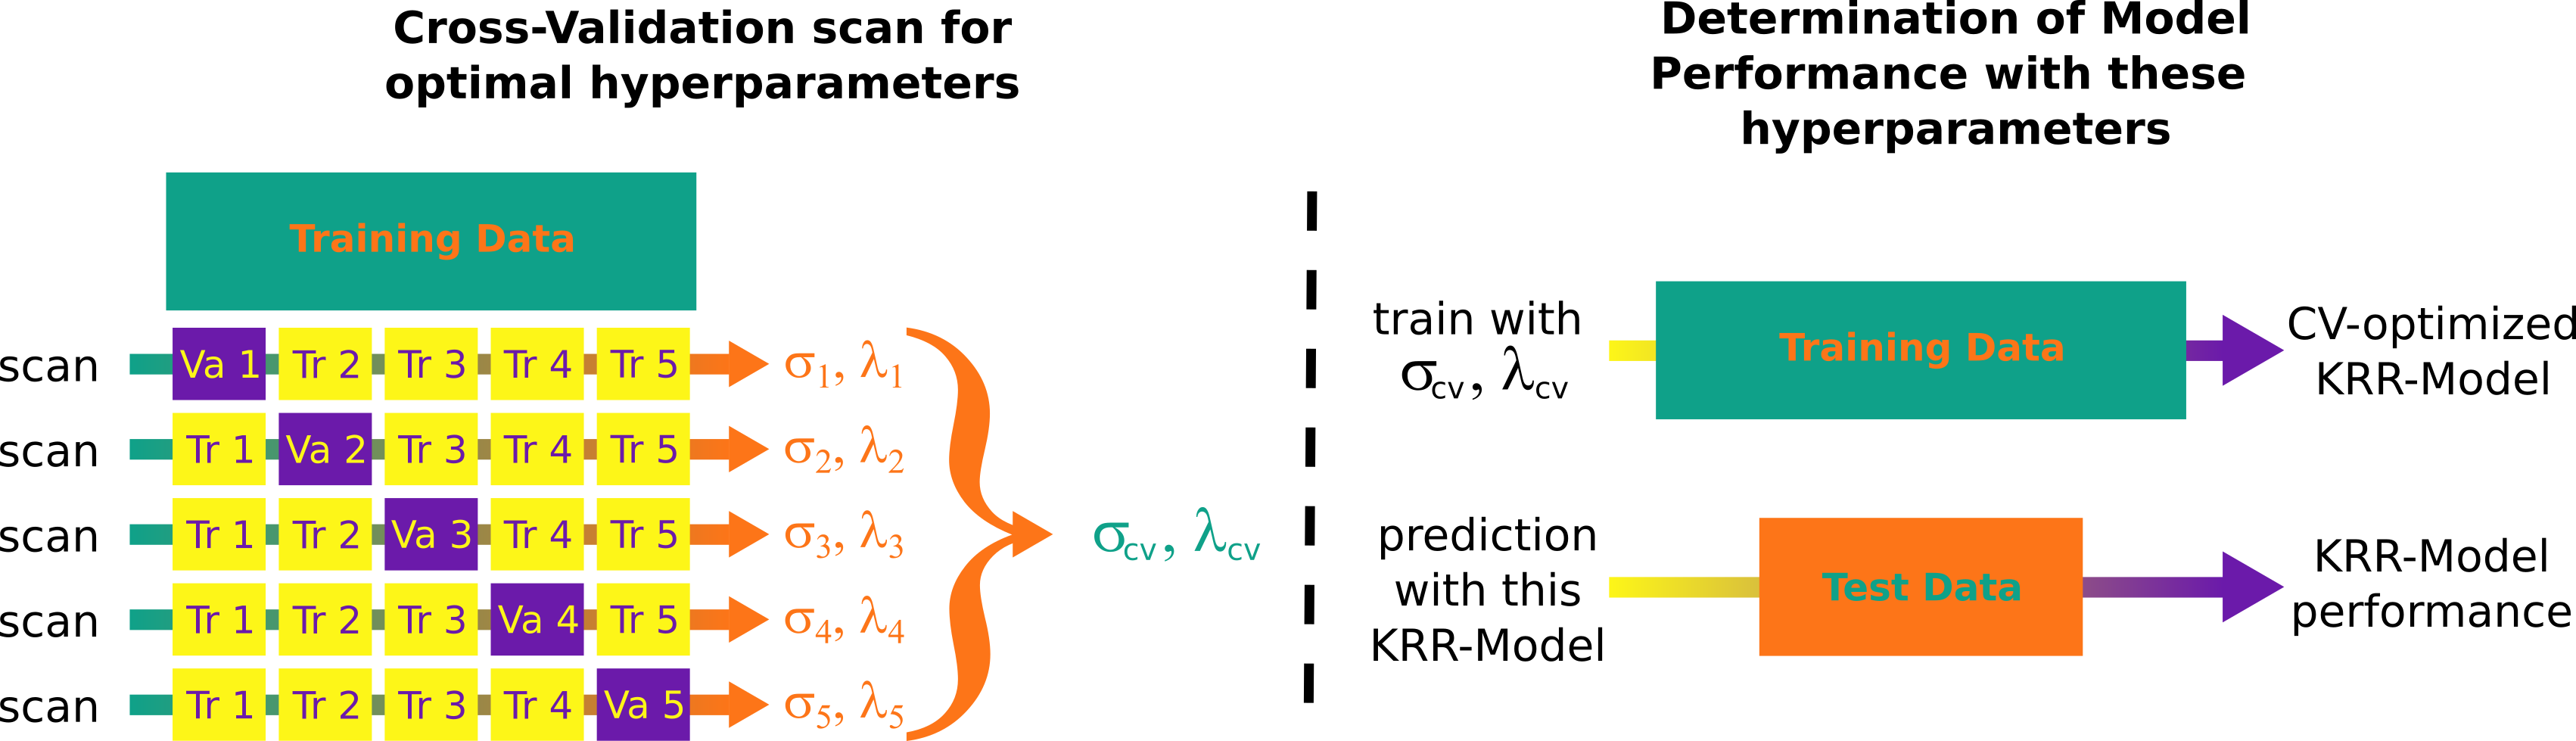
\includegraphics[width=16.5cm]{./resources/02_CV.png}
  \caption{(left) Training data broken down in $K$ (here five) blocks using stratification. Then, $K$ hyperparameter scans are performed, each time choosing one of the blocks as validation data (Va), while the rest remains as training data (Tr). (right) Model finalization with the obtained CV-optimized hyperparameters by training against the full training block. Then, determination of actual model performance by using this model for predicting the test data.}
  \label{FIG: 02_CV}
\end{figure*}

\noindent In each local scan of hyperparameters (i.e. each of the $K$ cross-validation steps), one of the smaller data blocks is chosen as the \textit{validation} dataset, whereas the remaining blocks become a local training set (not to be confused with the set of ``all known data used for training'', which includes also the testing data). This way, $K$ different optimal values for the $\sigma_g$ and $\lambda$ are obtained depending on which combination of validation and training set the model was trained on. Note, that inside each of the cross-validation steps we thus obtain a \textbf{locally optimal model} - which therefore suffers from overfitting with respect to the other validation blocks. The purpose of cross-validation is therefore two-fold: to find the best hyperparameters that also reduces overfitting through averaging over different cases. Note that this also shows that in machine-learning, optimizing for generality typically comes at the cost of accuracy and \textit{vice-versa}.

\noindent To train a most versatile model, we further must ensure that the training data in each cross-validation step evenly represents all possible values of the database. For example, it would be unwise to train a model on systems that have very high target values, when the overall distribution of data suggests that low values are more common. The process of distributing the data evenly into these $K$ blocks of training/validation data is called \textit{stratification} and can be performed by the \texttt{DataInst} object. Note, though, that stratification is \textit{not} to be applied before splitting the data in training and testing data. Ultimately, when the model eventually faces an unknown set of molecules, we are also unable to know beforehand if this set is evenly distributed or not. Therefore, we come closer to real prediction performances during the training procedure, if the test set is not part of stratification.

\paragraph{Options and methods of the DataInst object} -  Since the DataTens class features a larger amount of possible options, they are defined as class attributes. In the following the meaning and options will be explained. Note, that when we refer to ``training data'' in the following, we specifically mean the sub-portion of all data that is not the testing data. (since technically, both training and testing data is used for training, of course...)

\begin{itemize}
    \item \texttt{CVGridPts} - controls how many grid points are used for the optimization of the hyperparameters. This optimization needs to be carried out \textit{K} times during the \textit{K}-fold cross validation. Note that the required time for optimization with this grid-based method scales roughly with (\texttt{CVGridPts})$^2$, depending on the chosen optimizer.

    \item \texttt{CVSize} - controls the number \textit{K} of the \textit{K}-fold cross validation. This number thus controls into how many individual stratified blocks of data the active training data will be split during training - as well as how often ArchOnML expects to run hyperparameter optimizations. If you change this number, please remember that you will also need to change the number of times that you run the hyperparameter optimization with changing cross-validation blocks accordingly. The data blocks will be sorted (internally) into the objects' \texttt{DataInst.CVIDBlocks lists}.

    \item \texttt{RandomStrat} - controls the randomness during stratification (that is, sorting the data into the \textit{K} blocks). The random formulation will sort all data with respect to the specified stratification target, and then collect bins of size \textit{K} before randomly assigning these entries to one of the \texttt{CVIDBlocks}. Turning off randomness will always just sort the first value of a bin inside the first \texttt{CVIDBlocks} list and so on.

    \item \texttt{FixedSeed} - controls whether all randomness inside the class becomes seeded or not. Note, again, that even when using seeded randomness, each physical machine will still behave differently. During designing of your model / debugging we recommend to set this to true - and stick to one computer to see how changes affect your model performance in a direct way. To check robustness of your model, you may set it to false later to check how the model performs for different test sets.

    \item \texttt{MinMod} and \texttt{MaxMod} - These two \texttt{float} values are multipliers for the initial guess of the \texttt{sigma} hyperparameter. Internally, ArchOnML will guess initial sigma values for each descriptor (yielding an \texttt{array} of sigma values) - and each value will then be scaled according to these multipliers to give an upper and lower bound for the hyperparameter scan. This then leads to a \texttt{matrix} of sigma values with dimensions $N_\mathrm{Descriptors}$ by \texttt{CVGridPts}. Note, that in the current formulation of the model, the sigma value for each descriptor will be incremented together at the same time during the grid-based optimization - like one big hyperparameter. A completely flexible model, however, would require that each individual sigma for each descriptor needs to be scanned independently - leading to a computational training cost of \texttt{CVGridPts})$^{N_\mathrm{Descriptors}+1}$.

    \item \texttt{Lambda\_Bot} and \texttt{Lambda\_Top} - These two \texttt{float} values give the upper and lower scanned bounds for the lambda hyperparameter in terms of $10^\mathrm{Value}$. The use of lambda is, to account for noise in the training data. However, since the values are not actually from a measurement but a quantum chemical computation, noise should rather be understood as ambiguity. Still, from our experience, the optimal values for lambda are typically very small.

    \item \texttt{BinWinThrsh} and \texttt{BinWinEscape} - These two \texttt{integer} values control the behaviour of the internal method that estimates the initial sigma values for the descriptors. In short, the method tries to find the full width at half maximum around the most often encountered distance value for the descriptor by ``binning'' its distance matrix in histograms with a specified desired resolution of up to \texttt{BinWinThrsh} bins. The method will iteratively increase the bin-size - eventually ``escaping'' the iterations with the best values so far, if it can not reach a satisfactory result.
\end{itemize}

\noindent Finally, there is a memory option inside the DataTens class that differentiates between \textit{high}, \textit{medium} and \textit{low} memory modes. In \textit{auto} mode, it will attempt to choose the appropriate version based off your computer's architecture - however, you may also choose the version yourself. The three versions differ only in the sense that the lower you set the memory requirements, the more on-the-fly operations are performed (which consumes more calculation time).

\paragraph{DataInst.train\_test\_split(...)} - This method will organize the available data of the full training set into training and testing data. If only a single (float) number is given, it will assign random entries as training data until it fulfils the given percentage; and assigns the remaining entries to the test data.

\noindent If you do not supply a float number, but instead add the option \texttt{UPDATE=True}, you may provide a number to the option a \texttt{ActPerc} that will additionally set the currently selected training data to either active or inactive during learning. This way, you can steadily increase/decrease the amount of data you show to the model (while keeping the same test set!) to create a so-called learning curve for your model.

\paragraph{DataInst.stratify(...)} - This method stratifies the training data and sorts them into the \textit{K} blocks for the cross-validation. The method expects as input one of the previously defined label names (see \texttt{LLabelL}) in \texttt{string} (i.e. supplied with text in quotation marks!). Note that you can only stratify with respect to one target value  (i.e. label) at a time. Hence, while it is in principle possible to train a model against several target values at the same time, it is recommended to only train against a stratified set of data. Note, that stratification is only performed on the training data - and not on the test data of the model. This choice will make the final testing more realistic - since fully random test data is not necessarily evenly distributed.

\paragraph{Performing the cross-validation} - In the section ``Step 4'', the machine learning model instance is started and the cross-validation training is performed. For this purpose, you supply the IDs of the current validation data block and add together all other data blocks to give the training block. The number of blocks here depend on the selected \texttt{CVSize} (i.e. \textit{K} folds) that you defined. In general, a higher amount of \texttt{CVSize} is expected to produce a more generalized model - but may eventually spread your data too thin for meaningful training. Thus, careful balancing through trial-and-error is advised.

\noindent The actual hyperparameter optimization inside the current set of training and validation data is performed by the \texttt{KRR.cv\_para(...)} method. Currently, this method has three different optimizers with varying amounts of computational cost and accuracy. They will be briefly explained below - and in more detail in the developer's guide. Note that all of the optimizers will try to find a combination of hyperparameters considering fixed (but cross-validation data dependent) individual vectors for $\sigma_g$ plus one fixed vector for $\lambda$. For $N$ different descriptors, this spans a ``grid'' space of (\texttt{CVGridPts})$^{N+1}$ possible combinations. Also note, that the performance of a model is interdepently linked between dimensions. In other words, the optimum value for one descriptor $\sigma_g$ depends on the values of (possibly) all other hyperparameters.

\noindent The \texttt{optimizer="vectorized"} option, is the most basic option that will simply scale (simultaneosly!) all $\sigma_g$ while looping through all possible $\lambda$. Hence, the computational cost scales with only (\texttt{CVGridPts})$^2$. Since the initial guesses for the $\sigma_g$ are, however, motivated by the most occurring distances and its full-width at half maximum around it (see details in the developer guide), this optimizer is a good first guess for seeing if your desired model will be able to ``learn anything'' from the provided data. Below is what the output of the ``vectorized'' method looks like in the notebook.

\begin{figure*}
  \centering
   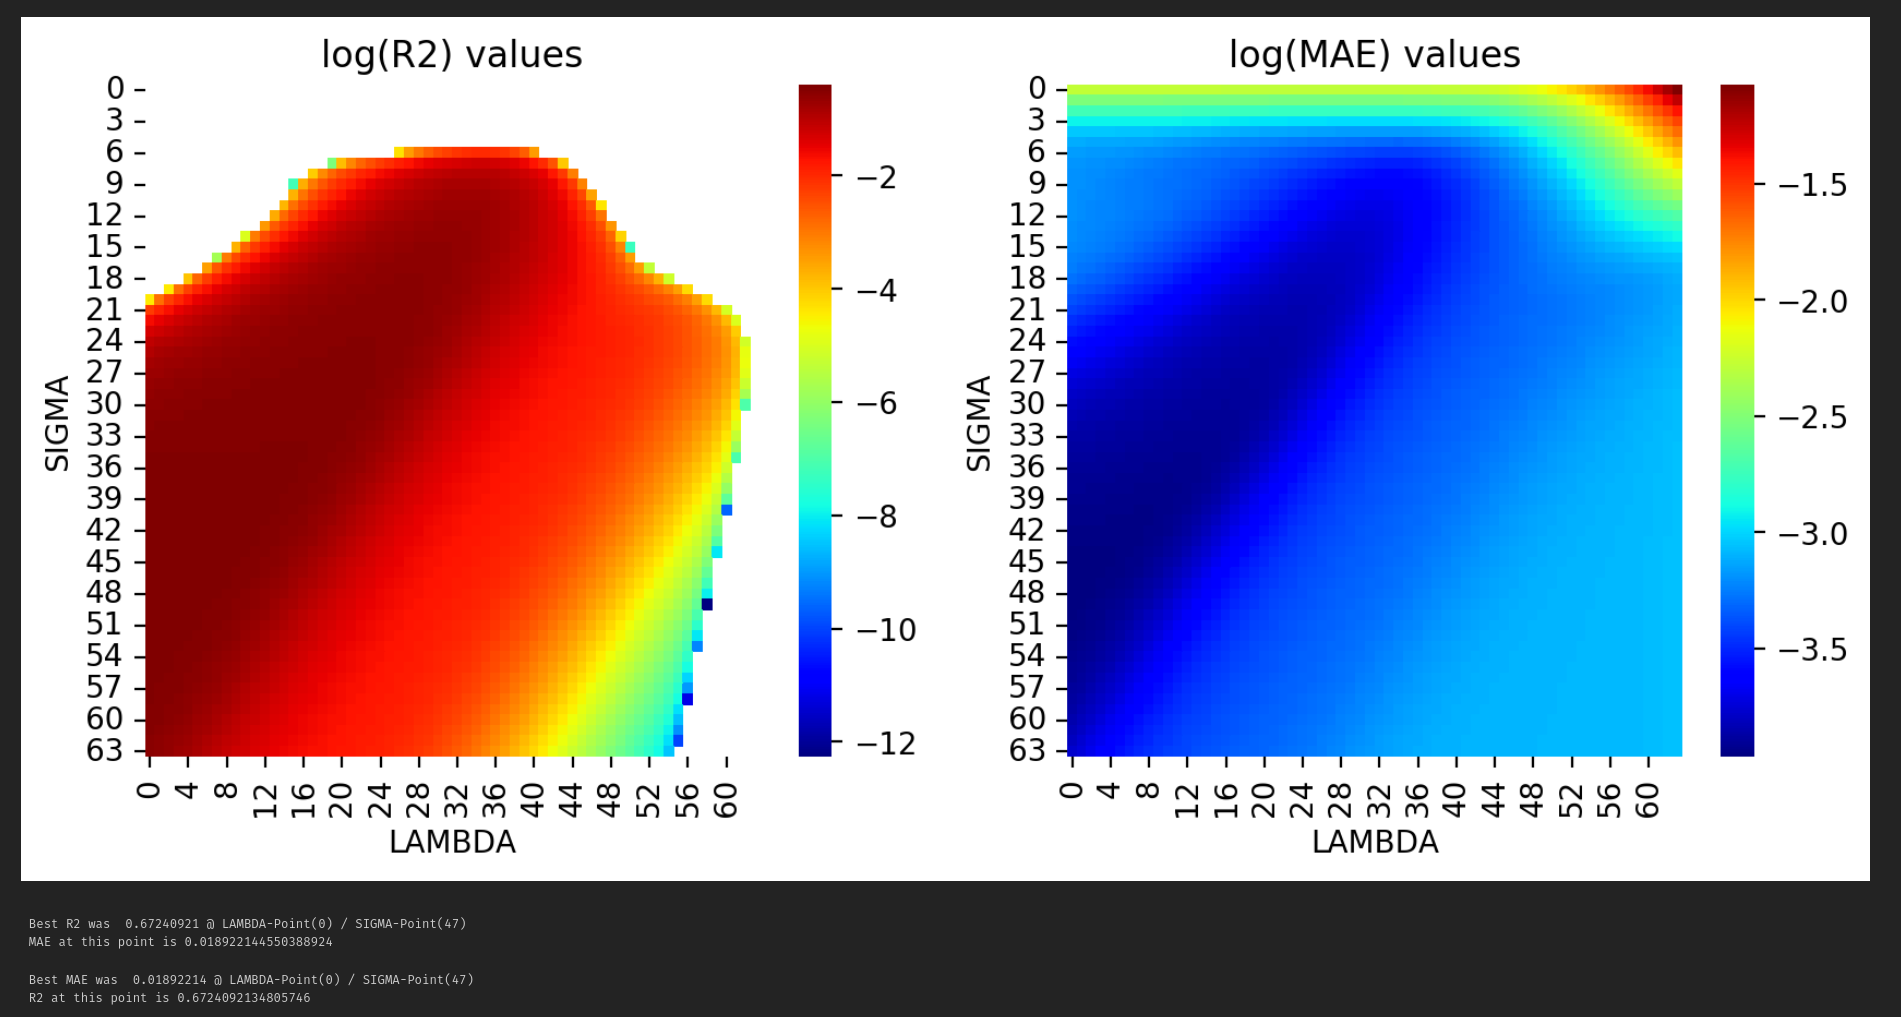
\includegraphics[width=15.5cm]{./resources/03_CrossValidation_Out.png}
  \caption{Output of one hyperparameter-optimizing cross-validation step. (left) logarithmic plot of the coefficient of determination (i.e. $r^2$) values of all models trained on the different hyperparameters. (right) logarithmic plot of the mean absolute error (MAE) on the same set of hyperparameters. (bottom text) Information on training statistics during hyperparameter optimization - best values encountered considering each plot individually.}
  \label{FIG: 03_CV_Output}
\end{figure*}

\noindent The other options will run a ``vectorized'' optimization first, and then further improve the hyperparameters from this initial guess. In the \texttt{optimizer="mean-field"} approach, individual 1D-scans along all $\sigma_g$ are performed (while freezing all other $\sigma_g$), storing all individual updates that would yield an improvement. After the scan, the optimizer then attempts to accept all improvements at the same time - which will yield in the optimal result, in case that the dimensions are not interdependent. Then, the optimizer will either (1) accept the globally improved version, (2) accept a single-dimension improved version or (3) reject any updates, depending on which of the three options shows the best performance.

\noindent The \texttt{optimizer="descent"} is an iterative improvement scheme that also starts from the ``vectorized'' initial guess, and then tries out (for all $\sigma_g$ and $\lambda$), all local 1-dimensional increases or decreases and stores the resulting performance. Then it chooses the best performing one and performs the same method until (1) a convergence criterion has been reached or (2) the maximum number of iterations has been reached. Note, that you can deactivate the check for convergence by setting the option \texttt{ignoreConv=True}, which may be useful in case that the initial guess starts in a ``very flat region'' of the $N+1$ dimensional landscape. Note that this optimizer will (in case of infinite iterations) always find a local optimum - without a guarantee that it is also the global optimum, though.

\noindent To rate the three optimizers in terms of accuracy, cost and robustness, the ``vectorized'' variant is surely the cheapest option with the least accuracy and robustness. The ``mean-field'' variant can potentially lead to the optimal model immediately and thus has a medium cost, high accuracy and medium robustness. Finally, the ``descent'' option (especially when forcing to ignore convergence) is a rather costly, however also highly robust and accurate method - that however \textit{can} become stuck in a local minimum.

\noindent Finally, when calling the \texttt{KRR.final\_cv(...)} method, it will put together the (thus far) collected optimized values for sigma and lambda and average them out over all cross-validation steps. Then, it trains the model one final time with these settings and predicts the data of the testing set (which the model still has never seen up to this point). The results of this finalization step give the actual performance of the model given the current training / testing data and hyperparameters. An example output of this is shown as a screenshot below.

\begin{figure*}
  \centering
   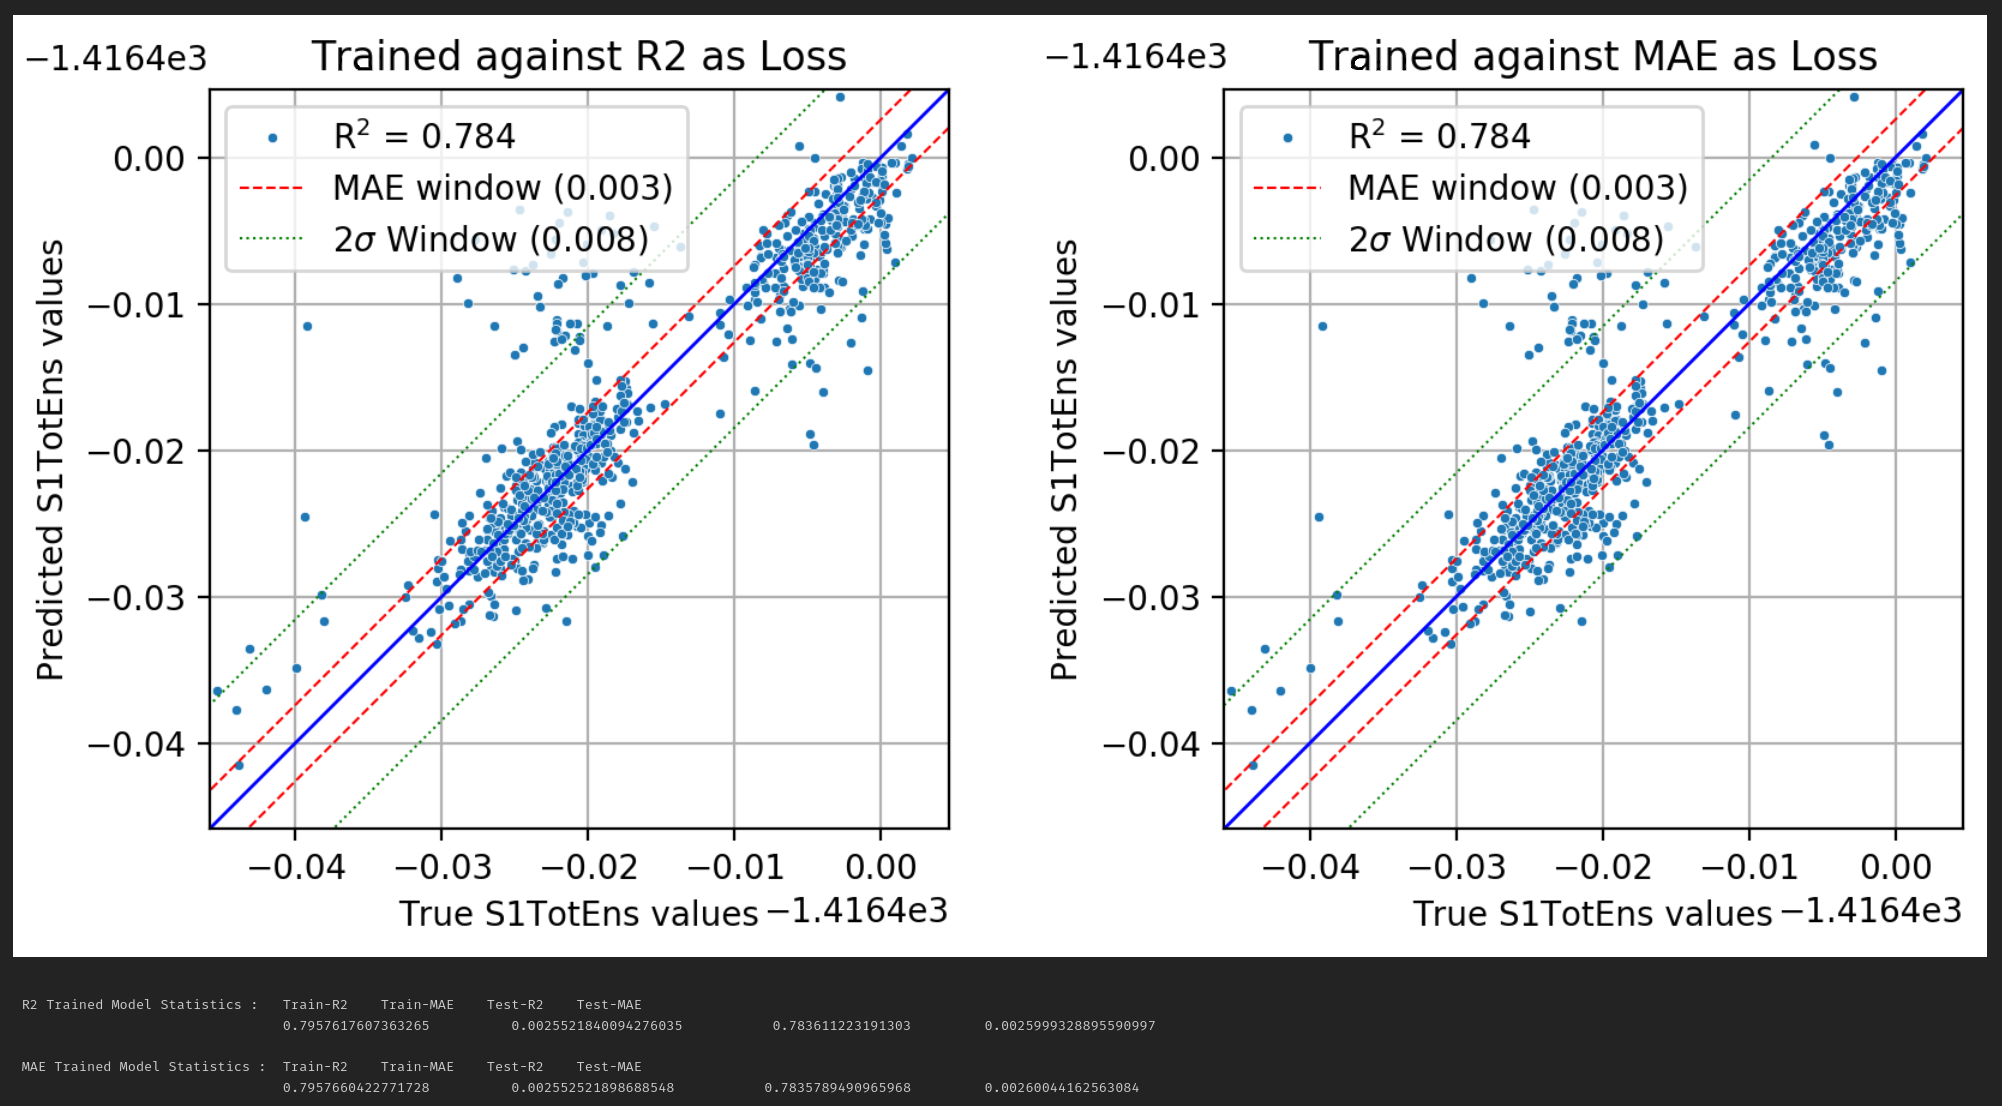
\includegraphics[width=12.5cm]{./resources/04_FinalCV_Out.png}
  \caption{Output of the model finalization step. Left (and right) shows the model performance at predicting the (thus far unseen) testing data with respect to a model which hyperparameters were optimized for $r^2$ (or MAE).}
  \label{FIG: 04_FinalCV_Out}
\end{figure*}

\noindent To check the robustness of your model, you should ultimately produce a learning curve by changing the active percentage (\texttt{ActPerc}) of training data - and eventually re-do several learning curves with also different testing sets of data, since maybe just a lucky test set was chosen at random. To do these statistics over different training / test sets, you can deactivate the \texttt{FixedSeed} option of the \texttt{DataInst} object and then perform a new \texttt{DataInst.train\_test\_split(...)}.

\paragraph{Saving the model} - If you are satisfied with your model after the \texttt{KRR.final\_cv(...)} you can save the finished model to hard disk for later predictions with the \texttt{KRR.save\_model()} method. Here, you may choose whether you want to store the best model based on the MAE or $r^2$ value. Per default, the better $r^2$ value is selected - but may be changed by setting \texttt{Loss} to either \verb|"R2"| or \verb|"MAE"|. By default, the models are saved inside the ``MLModels'' folder just above the ``Scripts'' folder. This location can be changed through adapting the class attribute \texttt{KRR.ModelPath}.

\paragraph{Running predictions} - Both the notebook ``02'' as well as the python script ``03'' contain the steps necessary for performing the predictions. In the beginning, ArchOnML will load the previously stored machine learning model that you specify. In case you changed the default saving location, make sure that you select it here again. While loading a model with \texttt{KRR.get\_model(...)}, ArchOnML will also load the training entries, hyperparameters and settings of the descriptor object instance that was used during training into a new \texttt{MLOBJLIST} and \texttt{DescInst}. This is necessary, since in kernel ridge regression, predictions are based off similarities of unknown molecules with the training set.

\noindent In the next step these (yet) unknown entries are loaded into the \texttt{MLOBJLIST} with \linebreak \texttt{LType=``Prediction''}. Needless to say, for all entries that shall be predicted, you need to have calculated all required raw data first. In other words, you need to have run semi-empirical calculations on \textbf{all} structures that you want to explore by prediction. Note that since these calculations require way less calculation time, you still end up with a worthwhile speed-up.

\noindent Loading the prediction entries is done by reading from a \texttt{SampleCalcs} file - just as for the training data. In case these entries have not been merged into native data format yet, you may on-the-fly perform the merging process through the \texttt{merge\_data()} method - which is by default commented out. After merging, you can then read in the raw data (\texttt{get\_merged\_data()}) and prepare the descriptors (\texttt{describe(...)}).

\noindent Finally, you need to initiate the data tensor object (\texttt{DataInst}) and run the prediction by calling (\texttt{predict\_from\_loaded(...)}). Note, that since the ``new data'' was flagged as ``Prediction'' data, both the \texttt{DataInst} object and the model object \texttt{KRR} know how to set up the kernel matrix for prediction automatically. Further, you may batch predictions into several independent predictions jobs on an hpc cluster by simply loading different \texttt{SampleCalcs} files in each predictor. Similarly you may just split any \texttt{SampleCalcs} file into many more such files to spread out the predictions more and more. 

\paragraph{Merging of several chemical spaces} - As briefly mentioned earlier, ArchOnML is currently not supporting the automatic generation of chemical spaces in which more than one substituent is bound to the same atom. In other words, there is no automatic generator for cases as the one below, where two substituent positions $R_1$ and $R_2$ are connected to the same carbon atom.

\begin{figure*}
  \centering
   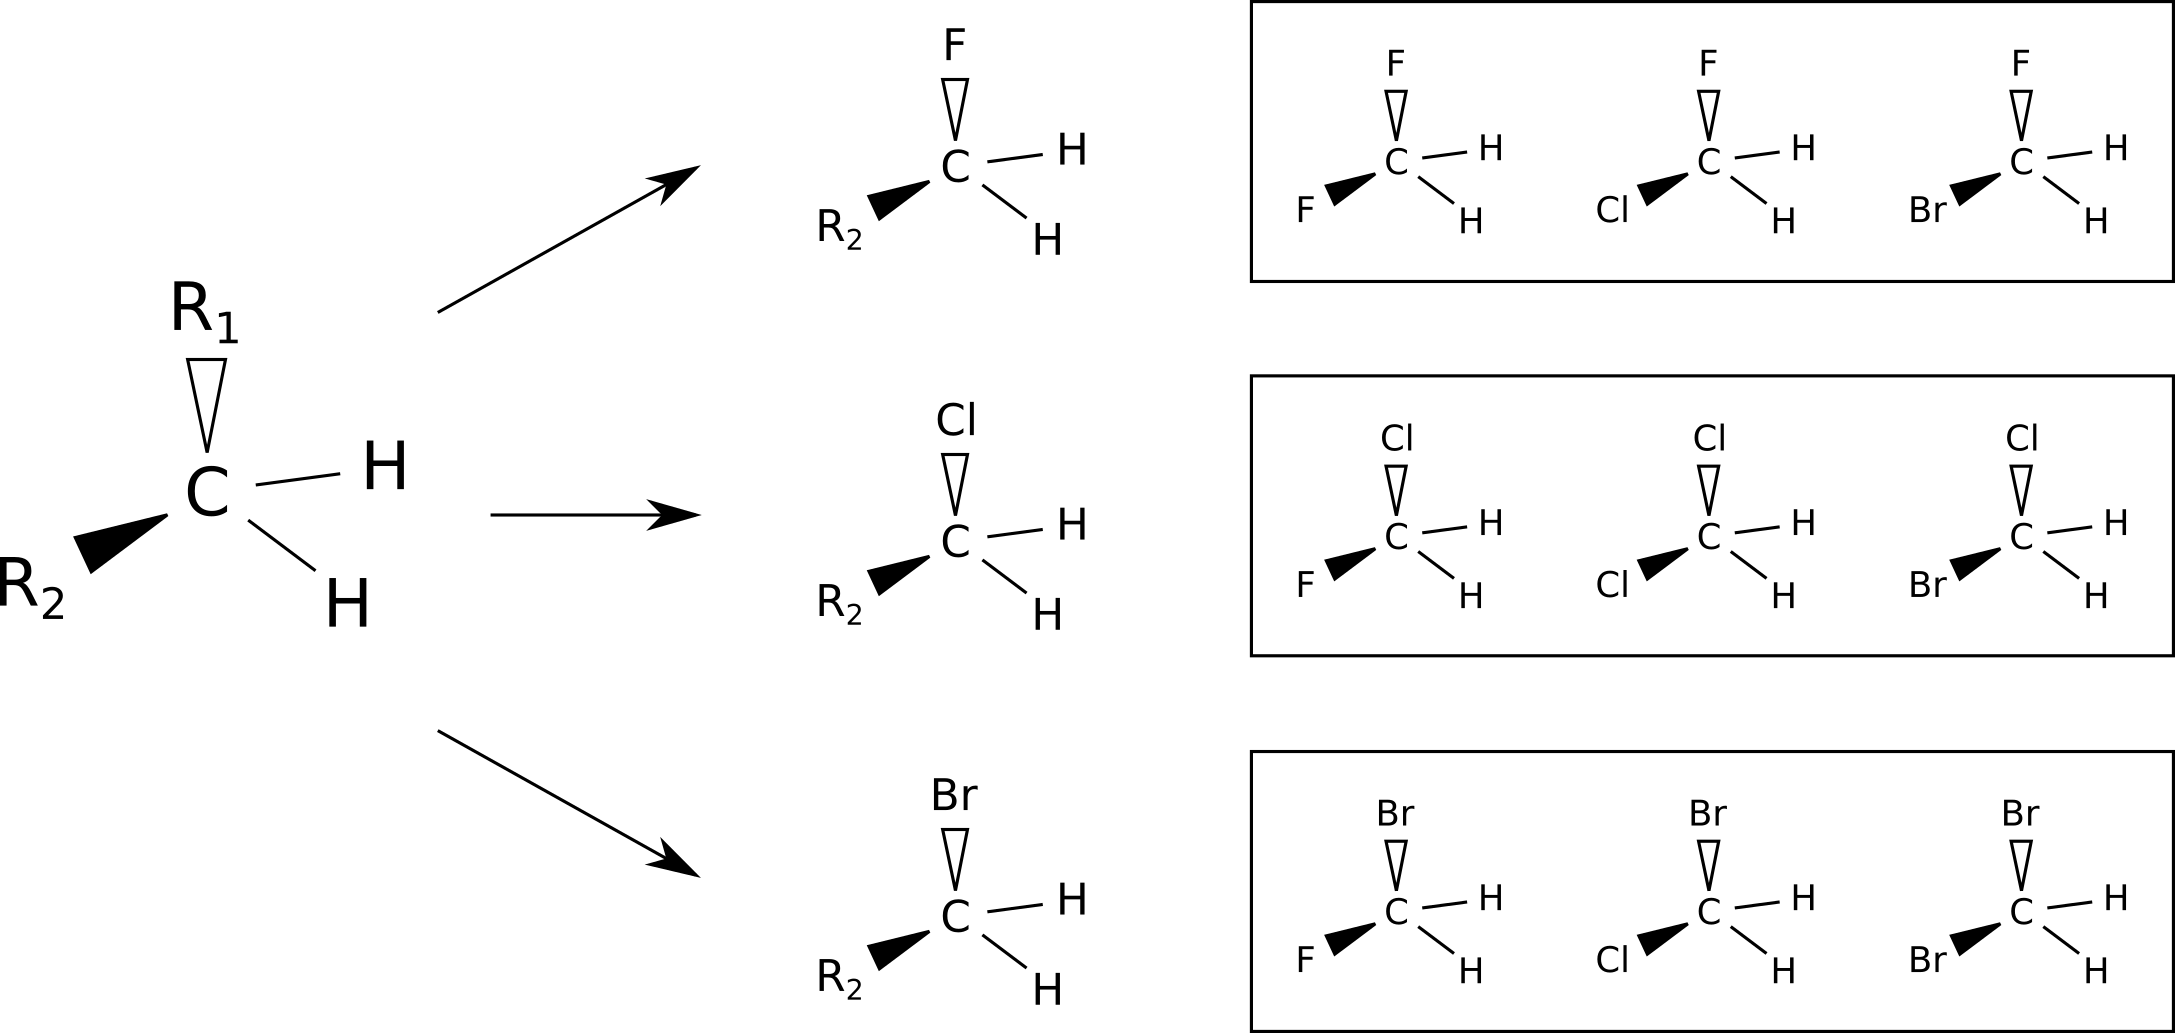
\includegraphics[width=12.5cm]{./resources/05_Merging_Spaces.png}
  \caption{Construction of the full chemical space by sub-spaces.}
  \label{FIG: 05_Merging_Spaces}
\end{figure*}


\noindent Assuming that you have three different substituents in your library (-F, -Cl and -Br), the currently implemented automatic generation \textbf{can} be used for the individual sub-spaces, however, where one of the substituents (here $R_1$) is fixed in its sub-space. Here automatic generation would then practically run over $R_2$, only. This can be easily achieved by using three different core structures. After each individual sub-space has been created, one must then check for symmetry equivalent structures in the whole space again, though. Note that in this simple example no \textbf{chirality} arises, which may be different for your specific case - and which is the main problem of why there is currently no automatic solution to these generation schemes, yet.

\noindent To then bring these structures together into ArchOnML we suggest to either develop your own fingerprint scheme by adding an additional information container about which ``local core structure'' was used - or just use the \textbf{conformation screening} notebook ``01b'' to set up the database by adding all generated \texttt{.xyz} files of the subspaces together into a ``conformers'' file. Note, that in this case you must keep a mapping of the fingerprints in mind, though, since notebook ``01b'' will not map the substitution pattern any more.

\subsubsection{Recommended Job Script Set-Up}

\noindent ArchOnML comes with several scripts for easy extraction of output data from the external quantum chemistry (QC) packages. These scripts can be found inside the \bl{Analysis} folder of the package, and are further subdivided for each currently implemented QC package. Note, that it is very useful to run some of these extraction scripts on-the-fly directly after the QC program finishes its calculation - especially for directly getting the ``PreOpted.xyz'' and ``Opted.xyz'' files from the QC outputs. If extracted directly, all generation steps of ArchOnML can proceed more smoothly. Note that, obviously, the extractor script could also be imported as a method of the MLEntry class to do the extractions in the interactive notebook - but currently this is not included, yet.

\noindent For example, if using a job-scheduling-engine like ``slurm'', you typically use so-called job-scripts to submit your QC calculations to be performed on the hpc cluster. Inside this script, you can directly perform the extraction script (plus any other analysis, if wanted) after each calculation is finished, by simply adding the python script execution to the job-script. Further, if your calculation task is set up in the form of a macro that uses a folder as its argument, you can directly transform the sample-calculations file into a job script. Below, a minimalist example for a ``PreOpt'' calculation with gaussian is shown for a ``slurm'' style job-script.\\

\newpage

\noindent\verb+#!/bin/bash+\\[-0.7em]
\verb+#SBATCH --ntasks=1+\\[-0.7em]
\verb+#SBATCH --cpus-per-task=1+\\[-0.7em]
\verb+#SBATCH --mem=640+\\[-0.7em]
\verb+#SBATCH --time=0-00:05:00+\\[-0.7em]
\verb+#SBATCH --job-name=PreOpt+\\[-0.7em]
\verb++\\[-0.7em]
\verb+# Below, absolute Path of the folder in which to+\\[-0.7em]
\verb+# start the job-script.+\\[-0.7em]
\verb+HUB=/scratch/user/MLProject/GENERATOR/Scripts/Calculations/01_PreOpts/+\\[-0.7em]
\verb++\\[-0.7em]
\verb+# MACRO TO RUN+\\[-0.7em]
\verb+MACRO(){+\\[-0.7em]
\verb++\\[-0.7em]
\verb+# Use "third argument" after "MACRO" to fill out $3 below+\\[-0.7em]
\verb+# Additional "../../" to account for additional relative pathing.+\\[-0.7em]
\verb+cd ../../$3/A_Geo_PreOpt_PM6/+\\[-0.7em]
\verb++\\[-0.7em]
\verb+g16 Geo_PreOpt.com+\\[-0.7em]
\verb+mv Geo_PreOpt.log Geo_PreOpt.out+\\[-0.7em]
\verb+formchk OPT.chk > /dev/null 2>&1+\\[-0.7em]
\verb+python ~/ArchOnML/PyPack/archonml/Analysis/gaussian/A_Extract_PreOpt.py+\\[-0.7em]
\verb+cp PreOpted.xyz ..+\\[-0.7em]
\verb+rm OPT.chk OPT.fchk+\\[-0.7em]
\verb++\\[-0.7em]
\verb+# The "tail" will push the last line of gaussian's output into a file namend+\\[-0.7em]
\verb+# Progress inside the "Calculation" folder+\\[-0.7em]
\verb+tail -n 1 Geo_PreOpt.out >> $HUB/Progress+\\[-0.7em]
\verb++\\[-0.7em]
\verb+}+\\[-0.7em]
\verb++\\[-0.7em]
\verb+# EXECUTE MACRO +\\[-0.7em]
\verb+# Below is then simply the SampleCalcs-File content plus "MACRO" written+\\[-0.7em]
\verb+# in front of each line.+\\[-0.7em]
\verb+MACRO AQ4698   2,4,2,2,1,2,1,3   ../../DATABASE/ANTHRA/2/2_4_2_2/ANTHRA4698/+\\[-0.7em]
\verb+MACRO AQ8916   1,1,4,2,3,3,2,2   ../../DATABASE/ANTHRA/1/1_1_4_2/ANTHRA8916/+\\[-0.7em]
\verb++\\[-0.7em]
\verb+...+\\[-0.7em]



\newpage
\subsection{3. Developer Guide to ArchOnML}

\noindent The following guide explains the intended purposes of each of the modules and classes of \linebreak ArchOnML while roughly following the workflow of the package. At specific points, explanations are provided on where and how to include new descriptors, interfaces to other packages or machine learning modules. Note that for any of the class methods, a \texttt{self} dependency was not explicitly written for the sake of brevity.

\noindent Note that the program code itself is also densely commented to explain what most of its lines do. Further, some modules like \texttt{utils.py} and \texttt{common.py} will not be explicitly described in here, since they mainly feature global definitions or general functions that will not further your knowledge on ArchOnML. If you have questions on how you might add a certain functionality to the code, you can contact us via github.

\subsubsection{The Generator Module / DBGenerator Class}

\noindent The Generator module (\texttt{generate.py}) has been designed to set up the third-party quantum chemistry calculation inputs and construct the initial (empty) database architecture. Further, it will generate all structural initial guesses in \texttt{.xyz} format. It contains the following functions, classes and methods:\\[-0.7em]

\dirtree{%
.1 generate.py. 
.2 rdgeom(path). 
.2 get\_repuls(GeomA, GeomB). 
.2 quater\_rot(Vec, Pos, Geom, Angle). 
.2 junction(CoreSubPos, CurFrag, CurrentCore, iCORE, iFLAGS, DBS=0). 
.2 full\_junc\_once(TUP). 
.2 class DBGenerator. 
.3 \_\_init\_\_(iProjName, iFragStrucLib, iCoreStrucFID, iStrucLib, iMergePath, iGuessPath, iDBPath, iFold\_L1, iFold\_L2). 
.3 gen\_fingers(). 
.3 gen\_db\_folders(). 
.3 sample(iSampLib, iLocSetLib, iNSamp, iFixedSeed=False). 
.3 gen\_calcs(iGenLib, iQCPack, iCalType, iCalFlav, iCalPathLib, **kwargs). 
}\vspace{1.0em}

\noindent First off, the purpose of the functions outside of the class is to generate the ``junctioned'' \texttt{.xyz} structures from the core structure and substituent files. Here, the main work is done by the \texttt{junction} function, which combines two \texttt{.xyz} structures by going through the following steps:

\begin{itemize}
    \item Aligning structures such that both $X\rightarrow{}Y$ marked bonds of the two fragments face towards each other by applying Rodrigues' Rotation theorem.
    \item Deleting the \verb+Y+ atoms and rotating around the newly formed bond between the fragments, using quaternions (i.e. the \texttt{quater\_rot} function).
    \item Calculating the (modified) nuclear repulsion between fragments with the \texttt{get\_repuls} function at each tested rotation.
    \item Returning the ``lowest repulsion'' structure as guess for the next junction step.
\end{itemize}

\noindent Note that the modified nuclear repulsion deliberately exaggerates the repulsion when atoms get too close, such that very light atoms don't accidentally become superimposed in the guess structures.  If you encounter such issues in your guess structures, you can try to change either the proximity threshold for the exaggeration or the additional multiplier (see ``\texttt{if Rij} $<$ \texttt{...}'' inside \texttt{get\_repuls}).

\noindent While aligning the two fragments an initial guess distance for the new bond is used, based on what atoms form the bond. These guess distances are stored inside the \texttt{PreDist} library of the \texttt{common.py} module. In this dictionary, atom labels have to be sorted from low to high atomic numbers. In case you need to define a new guess distance, you only need to add it to this dictionary accordingly.

\noindent Through the use of the \texttt{full\_junc\_once} wrapper function, one can serially junction all positions of the core structure. Note that the wrapper function is called in parallel mode in the IPython notebook to quickly generate all structures in RAM. If the sample size you choose to generate at once is too big to fit into your RAM, you may want to choose a lower sample size, instead. All functions have been written in a recursive way, such that the number of available substituent positions or the size of the fragment library is dynamically taken care of.

\noindent Next, the class \texttt{DBGenerator} is introduced. To configure all its methods, it is initialized as an object by providing the core structure, a library file of fragments and further general information about the planned project's location on the computer. During initialization it will also write this information to a file called \verb+DBSpecs.cfg+, which should not be changed afterwards. Here, it will also save whether a chemical space screen or conformational space screen is to be performed, which will affect the behaviour of all code sections that work with the fingerprint of any entry.

\noindent From the core structure and fragments, the class' \texttt{gen\_fingers} method is able to recursively generate all permutations of possible substitution patterns in numerical code format (i.e. [1, 6, 1, 4]). These codes are referred to as fingerprints. Note, that \texttt{gen\_fingers} does not take into account symmetry elements in the core structure. Hence, to avoid double-counting inside the database, you need to remove symmetrically equivalent fingerprints by providing redundancy rules. The notebook contains an example on how rules can be given in a brute-force approach. In case of a conformational space screen, the meaning of the fingerprints changes to just pointers for the folder structure and the \texttt{n}-th ``frame'' that was taken from the provided \texttt{ConformerStrucFID}, containing all conformers.

\noindent After the fingerprints are created (and have been reduced with respect to symmetry or any other desired generation rules), the \texttt{gen\_db\_folders} method creates the three main folders and sub-folders required for the molecular design project: One for calculations with the third-party quantum chemistry package (called \texttt{DBPath} in the ``01'' notebooks), one folder hierarchy to store the initial guess structures in (called \texttt{GuessPath}) and one folder hierarchy where the raw data of semi-empirical calculations is collected (called \texttt{MergePath}).

\noindent The purpose of collecting the semi-empirical raw data is, to save all information that is required to construct your desired descriptors in one file with a native format. This way, all other procedures in ArchOnML become independent on the exact output format of the third party quantum chemistry program packages. Further, storing the outputs of different calculation files into one file can drastically reduce the amount of input / output operations per entry - and also allows to delete all of the external programs' (usually larger) output files to save hard disk space.

\noindent For the hierarchy structure of the folders, two levels of sub-folders are created. The reason for this is, that data look-up becomes extremely slow, when there are several thousands of files or folders inside one folder. Thus, using a number of branching sub-folders increases the speed of storing and loading data later on. The depth of these structures is given by the class attributes \texttt{Fold\_L1} and \texttt{Fold\_L2}. The branching follows the fingerprint logic - i.e. using \texttt{Fold\_L1 = 1} and \texttt{Fold\_L2 = 2}, a structure with fingerprint [1, 6, 1, 4] is found in folder \texttt{1/1\_6/}. Finally, the entry's ID will be used to generate it's so-called \textit{stem folder}, in which the calculations and structures will be collected for the third-party calculations. Assuming that the internal ID of fingerprint [1, 6, 1, 4] was \texttt{PROJ126}, then it's calculations will be found inside the stem folder \texttt{../../DATABASE/PROJ/1/1\_6/PROJ126/} (depending on what your \texttt{DBPath} was set to).

\noindent Next, the \texttt{sample} method of the \texttt{DBGenerator} instance can be used to get a number of random samples from all available entries. This is useful for preparing the calculations of your training data in randomized batches of manageable sizes and to increase your training data in a step-wise manner. For each sample, a file (with a name specified in \texttt{LocSetLib}) is created, that contains information on which entries are in this sample. This file is later used to generate the input for the quantum chemistry calculations - so you should change the name for each new sample. Also, the method will store all entries that have been sampled before inside the a file that is specified under \texttt{SampLib}, such that calling the method several times will not result in double counting. Needless to say, this file name should not be changed after setting it for your project, since otherwise you lose track of what has been done already.

\noindent Finally, the \texttt{gen\_calcs} method takes one of the specified sample files (i.e. a previously created \texttt{LocSetLib}) and generates the inputs for the quantum chemistry calculations. The method requires further keywords on what external software shall be used and what calculation is to be performed. Note that ArchOnML works with a logic of pre-defined calculation types and flavors, since calculations should be highly standardized anyway to ensure that all database entries have been treated in \textit{exactly} the same way.

\noindent Here, a \textit{calculation type} conveys what calculation should be performed - e.g. a structure \linebreak (pre-)optimization or excited state calculation, etc. The \textit{calculation flavor} then specifies \textit{how} the calculation should be performed - e.g. what method (i.e. DFT functional) and basis set are to be used. As mentioned, both types and flavors are currently associated with pre-defined keywords, to provide a streamlined input in ArchOnML across the interfaced quantum chemistry packages. Therefore, the \texttt{gen\_calcs} method calls upon another separate module inside the \texttt{calcgen} sub-package, depending on which quantum chemistry code is used.

\paragraph{Parsing the Input - Calculation types and flavors} The calculation types and flavors are managed in the \texttt{calcgen} sub-package, where for each external quantum chemistry code there is a separate module. These contain the \texttt{GenInp} function as well as package-dependent definitions of calculation types and flavors. Which of the modules is imported inside the \texttt{DBGenerator} depends on which \texttt{QCPack} was specified.

\noindent Calculation types are stored as dictionaries that contain a folder name, input and output file names, a dummy string and a geometry flag. Each calculation type should be connected to its own folder name, to keep calculations well-separated. Remember that at several hundreds of thousands of calculations, you can not easily check individual calculations any longer, so, generality and transportability need to be ensured at the lowest level possible.

\noindent The dummy string contains the input commands for the calculation, with placeholders for the flavor (e.g. basis sets and further keyword arguments like the number of excited states). Finally, the geometry flag specifies what geometry is used for generating the calculation input. It has three options (\texttt{Guess}, \texttt{PreOpted} and \texttt{Opted}) and will use the respective \texttt{.xyz} file inside the \texttt{stem folder} to complete the input file. For screening a conformational space, you should use \texttt{Guess} for your follow-up calculations, assuming that the structures provided inside the \texttt{ConformerStrucFID} are (pre-)optimizied already in some way.

\noindent Similarly, calculation flavors are also dictionaries that contain fixed method and basis set information, that should (by design) not become flexible unless you change to a different flavor (which results in a new calculation folder). The idea behind this is, to then use one flavor across several calculation types consistently.

\noindent For both orca\cite{orca_cite} and gaussian\cite{g16_cite}, the \texttt{GenInp} function will construct the input files by combining the dummy string of calculation commands with the \texttt{.xyz} data. Other external programs may require different input styles, but the general set up should be followed, if possible, in similar ways. In case you want to add a new program package, you should thus start by copying and modifying one of the sub-package modules and then add the package's name to the \texttt{DBGenerator} class to load your desired input parser.

\noindent To define a new calculation types or flavors, new dictionary entries need to be added to the respective \texttt{CType} or \texttt{FType} dictionaries. For this purpose, you can just copy and modify any existing types and change their name inside the dictionary. Make sure, though, that your calculation type is robust in the sense that you have tested it for a few of your structures to avoid submitting thousands of calculations that will run unstable. 

\noindent To interface ArchOnML to a new external quantum chemistry package, you first need to understand how the input needs to be provided for the new program suite. While \texttt{orca} and \texttt{gaussian}, for example, work with stand-alone input files that contain all information for one calculation in one file, other programs such as \texttt{turbomole}\cite{Balasubramani_2020} rely on an indirect input style. Here you (usually) use the \texttt{define} routine of \texttt{turbomole} to set up the calculation in an interactive way. To set up an appropriate parsing interface with ArchOnML, you may thus want to generate an interim ``input file'' for running \texttt{define} instead.

\noindent After figuring out the necessary input style, you may then copy and modify an existing module in the sub-package \bl{calcgen}, add your desired calculation types and flavors and add the option to use this program package inside the \texttt{generate.py} module. You may want to add a comment somewhere for which prorgam version your new parser was developed for, such that new users may eventually copy your parser from the github, if you decide to contribute to the project.

\noindent Interfacing a new program package will also require you to add a parser for translating the outputs to ArchOnML's native raw data format. There will be some explanations on how to do this below.

\newpage

\subsubsection{The Entries module}

\noindent The Entries module (\texttt{entries.py}) contains the following class and methods:\\[-0.7em]

\dirtree{%
.1 entries.py. 
.2 class MLEntry. 
.3 get\_db\_specs(). 
.3 \_\_init\_\_(iID, iType, iFingerP, iQC\_Pack, iQC\_low, iQC\_high, iDataL, iLabelL). 
.3 merge\_data(). 
.3 get\_merged\_data(). 
}\vspace{1.0em}

\noindent The purpose of its \texttt{MLEntry} class is, to provide an object designed specifically for transporting and storing all information on the individual entries of the database. An individual object instance is initialized by providing it with

\begin{itemize}
    \item the entry's ID (e.g. \texttt{PROJ4290}). Required for locating the \texttt{stem folder}.
    \item the type of entry - i.e. whether it is used for \texttt{Training} or \texttt{Prediction}. This information will affect the behaviour of the \texttt{DataTens} class, and whether to look for a label value from a file or not.
    \item the entry's fingerprint. Required for navigating folder paths.
    \item the quantum chemistry package that was used in the calculations. Used to select the correct parser of the output files.
    \item the flavor used for calculating the low-quality data (e.g. ``PM3''). Used to construct folder names.
    \item the method used for calculating the label values - currently unused by ArchOnML.
    \item a list identifiers for which raw data is to be taken from the low-quality calculations. Used in determining what files to open for (and what output to use in) merging data into the native format.
    \item the list of label names that shall be looked for and added to the entry.
\end{itemize}

\noindent Using the specifications stored in \texttt{DBSpecs.cfg}, the class is able to identify the \texttt{stem folder} that belongs to the entry (i.e. the one containing all calculation folders), so that it can collect all raw data of the entries. You can use the \texttt{get\_db\_specs} class method to read in an existing \texttt{DBSpecs.cfg} file and use it on all \texttt{MLEntry} objects.\\

\noindent Depending on which quantum chemistry package was used (i.e. \texttt{QC\_Pack}), the object instances can turn their semi-empirical quantum chemistry output into ArchOnML's native format by using the \verb+merge_data+ parsing method. This raw data file is stored inside the \verb+SemiEmpData+ folder hierarchy, such that the quantum chemistry outputs can (in principle) be deleted afterwards for reducing hard disk space. A special section on how to set up a parser for the native file format is provided below.

\noindent After assigning which raw data shall be used, the data can be collected from the quantum chemistry output and stored inside ArchOnML's native format via the \verb+get_merged_data+ method. Note, that this has to be performed only once.

\noindent Finally, note that both the low-quality method (\texttt{QC\_low}) and the program package specification (\texttt{QC\_Pack}) are not class-wide attributes, but instead attributes of each individual instance. In other words, it is possible to use entries from different quantum packages and/or different low-quality methods inside the same database.

\paragraph{Parsing the Output - The native file format}

\noindent ArchOnML was designed with the goal to only introduce parsers for external quantum chemistry packages at two different interfaces - once for generating input files for the programs (as managed inside the \texttt{gencalc} sub-package mentioned above) and once for reading the raw output, which is later turned into all kinds of descriptors.

\noindent The currently used native format uses a block form, where each data block carries a chunk of (shortened!) output that can be collected from different calculation types' output files. Currently, this information is limited to structural information, Mulliken charges at each atom, as well as information on the semi-empirical orbital energies and shapes - however, we highly encourage users and developers to include their own data blocks for increasing the scope of possible descriptors in the future.

\noindent If you are including your own data blocks, you should make sure that the new blocks don't interfere with old ones. To make room for this, the MLEntry currently uses a so-called \textit{data list} (i.e. \texttt{DataL}) with keywords that will trigger reading (or writing) specific blocks of data from (or to) the merged files. Keep in mind, though, that the main goal of the native format has to be data reduction - so that no excessive amount of data should be stored from the raw outputs.

\noindent If you are interfacing a new external quantum chemistry package for ArchOnML, you will need to write a parser that will (exactly!) re-create the output format as shown in the provided example file available inside the \bl{Sample\_GENERATOR} folder. Since the native format is originally derived from the \texttt{gaussian} output style, you can take ideas of how to achieve your own parser from the existing \texttt{orca} one. Notable differences in the output styles (that may become a pitfall) here, are that \texttt{orca} will start counting molecular orbital IDs from zero, while gaussian starts from one. Further, the molecular orbital section (which gives the molecular orbitals in terms of atomic orbital coefficients) of \texttt{orca} will typically have 5 columns of molecular orbitals, while \texttt{gaussian} features 6.

\noindent Future versions of ArchOnML will also include a parser for the \texttt{molden}\cite{Schaftenaar_2017} format that has a lot of transportability between program packages and post-processing packages already.

\subsubsection{The Descriptor Tools module}

\noindent The descriptor tools module (\texttt{desctools.py}) has a single class called \texttt{Descriptor} with a method called \texttt{describe}. The class was designed with the purpose to allow initializing an object, that ``looks'' at an object of the \texttt{MLEntry} class and ``describes it'' by attaching the user-requested descriptors to it.\\[-0.7em]

\dirtree{%
.1 desctools.py. 
.2 class Descriptor. 
.3 \_\_init\_\_(iDescL). 
.3 describe(MLEntryObject). 
}\vspace{1.0em}

\noindent By providing the list of keywords in the \texttt{DescL} list, the object automatically builds the \texttt{describe} method in the necessary way. Here, for each descriptor, two additional pieces of meta-data are attached to the MLEntry object in the form of the \texttt{DescType} attribute. These store firstly, what kind of data (i.e. format) the descriptor is (on position 0 of the list) - i.e. a ``Scalar'', an ``Array'', an Array-of-Arrays or more specific types such as a Coulomb Matrix(-like) object.

\noindent Secondly, it carries information on what should be done with this data for determining the similarity between two entries (on position 1 of the list). Here, there are simple operations such as ``DistMat'' that will just calculate the difference between the two respective values directly, and more intrivate pones like ``EucDistMat'' that will prompt the calculation of the Euclidean Norm (in a specific way, see reference\cite{Rupp2012}) for the ``distance'' between two molecules. Note that forming distance matrices may not be required for other machine-learning models than Kernel Ridge Regression, but giving the full definition will make it available to KRR and eventually other models, anyway.

\noindent Note, that the design choice of assigning descriptor data and meta-data at the same step allows for better transportability, since new descriptors need to be defined only inside the \verb+desctools.py+ module - as all other modules and objects don't require information about how any descriptor was determined - but rather, only what the data looks like and what should be done with it. For easier readability, functions that are used for post-processing the raw data to obtain descriptor values have been moved into the general \verb+utlis.py+ module.

\noindent In case you want to define a new descriptor within the existing data formats and distance matrix-related operations, you can simply add a new \texttt{if} statement for your new descriptor's name and add how to obtain the descriptor value f(A) the generation of the chemi-
cal space, (B) calculation of the training set data, (C) training
and validating the ML model and (D) performing the predictions
and analysis. rom the available information inside the \texttt{MLObject}.

\noindent Outside the existing data formats and operations, there will be a few more places besides the \texttt{desctools} module that will require the new definitions. For one, the \texttt{krr\_tens.py} module will need the new formats and operations - here you can search for the keywords \texttt{DataF} and \texttt{DataO}, respectively, to find where changes will be necessary.

\noindent The \textbf{same} changes unfortunately need to be made additionally in the ``low'' and ``medium'' memory sections of the \texttt{utils.py} module, as well as the \texttt{krr\_model.py} module. The reason is that right now in the other memory modes, different objects will assume the responsibility of calculating the descriptors on-the-fly. This will eventually become more uniform in future updates to ArchOnML again.

\subsubsection{The DataTens Class}

\noindent After the list of MLEntries (called \texttt{MLOBJLIST} inside the notebooks) has been fully described, the \texttt{DataTens} class generates and manages the distance matrices of the \textit{abstract distances} required for kernel ridge regression. Note that this class is only really useful if you are planning to use a kern(A) the generation of the chemi-
cal space, (B) calculation of the training set data, (C) training
and validating the ML model and (D) performing the predictions
and analysis. el ridge regression (KRR) machine learning model. It is initialized by providing the \texttt{MLOBJLIST} directly.\\[-0.7em]

\dirtree{%
.1 krr\_tens.py. 
.2 class DataTens. 
.3 \_\_init\_\_(MLOBJLIST, mem\_mode="auto"). 
.3 train\_test\_split(iPerc, UPDATE=False, ActPerc=1.0).
.3 stratify(iLabelL). 
.3 update\_cv\_tens(TrainIDs, ValiIDs, MLObjList=[]). 
.3 final\_tens(TrainIDs, TestIDs, MLObjList=[]). 
.3 get\_pred\_tens(MLObjList, TrainIDs, PredIDs, Sigmas). 
}\vspace{1.0em}

\noindent Upon initialization, it will read all relevant meta-data of all entries (IDs, fingerprints, type (\textit{Training} or \textit{Prediction}), as well as descriptor lists and their types). On \texttt{"high"} memory setting, it will then proceed to pre-calculate the full distance matrices for all descriptors as look-up tables using the MLEntry's descriptor list (\verb+DescL+) and their attached meta-data (\verb+DescType+). The other memory settings will be explained closer to the end of the section. After the full distance matrices have been built, there are some methods for managing the data contained within the object.  

\noindent Firstly, for training a KRR model, it is necessary to split the data into training and testing sets. This is performed by the \texttt{train\_test\_split} method. The method will randomly assign the status \texttt{TrainActive} or \texttt{Test} to all entries that have been marked as \texttt{Training} previously. Note, that there are different options on how to treat the randomness of this step - either by using a fixed seed or not. Further note, that a fixed seed setting will still produce different results on different machines, as the artificial randomness is still hardware dependent. The type of randomness can be changed with the boolean class attribute \texttt{FixedSeed}, which is by default set to True.

\noindent Afterwards, you can decide to use only a portion of the training data for the following cross-validation steps - which is necessary if you want to produce a learning curve of your model. To do this, the \texttt{train\_test\_split} method can be run with the option \texttt{UPDATE=True} and a percentage value of how much of the training data should be set to ``active''. Note that this will \textbf{not} affect the already performed split into test and training overall - which is of course desired as a learning curve only makes sense if training is compared for a fixed test data set.

\noindent Next, the \texttt{DataTens} object can be used to stratify all active training data into $K$ sub-sets of same length - which is required for the following cross-validation method. Stratification means that all possible label values are first sorted, and then evenly (but randomly) put into $K$ bins, with the purpose that a number of $K$ subsets with similar target data distribution is obtained.

\noindent The $K$ sets of data can then be used directly for the $K$-fold cross-validation for optimizing the hyperparameters of the KRR model (a detailed explanation on what that means follows in the section below). For each step of the cross-validation procedure, new distance matrices must be collected and embedded into a the kernel matrices for training and validation.

\noindent On \texttt{"high"} memory setting, the distances were pre-calculated at initialization, and thus the distance matrices for the current cross-validation set can be looked-up by the \texttt{update\_cv\_tens} method in relatively short time. On \texttt{"medium"} memory setting, no look-up table was produced - but instead, the distance matrices of all descriptors are calculated only when starting a cross-validation block.

\noindent On \texttt{"low"} memory setting, no distance matrices are stored at all, and only when a descriptor is being evaluated, it will be generated for that instance. Note that this makes training extremely slow - but will only require a few hundred megabytes even for thousands of training entries and dozens of descriptors.

\noindent Here, for each step of the cross-validation procedure, the method is provided with only the (numerical) IDs of the blocks that are to be used as training and validation data. The method also constructs the dynamic range for the hyperparamater scan of $\sigma$ - which is explained in detail inside the MLModel Class section, below. 

\noindent The remaining two methods \verb+final_tens+ and \verb+get_pred_tens+ are also not directly called by the user, but rather are used directly by the MLModel class, described below. Hence, their explanation will also be given below as well, to stay in chronological order of the workflow. 

\subsubsection{The MLModel Class}

\noindent The \verb+MLModel+ class of of the \verb+krr_model+ module is the main driving object for running all ML related processes.\\[-0.7em]

\dirtree{%
.1 krr\_model.py. 
.2 class MLModel. 
.3 \_\_init\_\_(iLabel). 
.3 cv\_para(DataTensObj, MLObjList=[], optimizer="vectorized", convR=0.005, convM=0.0001, MaxIter=100, ignoreConv=False).
.3 final\_cv(DataTensObj, MLObjList=[]). 
.3 save\_model(iName, Loss="R2", Method="Auto"). 
.3 get\_model(iName). 
.3 predict\_from\_loaded(DataTensObj, MLObjList). 
}\vspace{1.0em}

\noindent The \verb+cv_para+ method runs one full hyperparameter scan in parallel mode. To do this, it uses the entries currently assigned to the Training and Validation blocks of the \verb+DataTensObj+ object - which is why these need to be updated before each call of \verb+cv_para+. The range of hyperparameters $\sigma$ and $\lambda$ that is scanned is also stored inside the \verb+DataTensObj+ attributes. Here, values for $\lambda$ between $10^{-6}$ to $10^{2}$ are scanned by default. The hyperparameter $\lambda$ is the so-called regularization strength and can be understood as a switch that controls how much variance is expected inside the data. In other words, low values will result in strict models that treat the training reference as being free of noise. As the training data is obtained from computational rather than analogue experiments, this hyperparameter is typically expected to be rather low - however, its inclusion can nonetheless improve results accounting for the approximations made in (semi-empirical) quantum chemistry.

\noindent The range for $\sigma$ is dynamically guessed at each update of the cross-validation block (the details of this guessing procedure will be given further below). As explained earlier, a KRR model will derive the predicted value for an unknown entry based off its similarity to a reference set of entries with known solutions and trained weights. Here, similarity is determined by comparing \textit{abstract distances} $d_g (M', M_i)$ between pairs of molecules $M'$ and $M_i$ for different properties $g$ (i.e. the \textit{descriptors}). Currently, the implemented KRR model will determine each descriptors' similarity using the so-called \textit{gaussian kernel}. Here, the similarity between two molecules is a number between 1 and 0, given by the exponential expression:\\[-3em]

\begin{equation*}
    f(M_i, M_j) = \exp \Bigg(-\Bigg( \sum\limits_{g}\frac{d_g(M_i, M_j)^2}{2 \sigma_g^2}\Bigg)\Bigg)
\end{equation*}

\noindent Hence, the meaning of $\sigma_g$ is a width parameter for the gaussian of each distance $d_g$. When calling \texttt{update\_cv\_tens}, only the distances relevant for the respective training blocks of the cross-validation are picked from the full collection of distance matrices. Next, from these entries, histograms of the distance matrices for each descriptor $g$ are formed. These histograms contain all encountered abstract distances $d_g$ and their distribution.

\noindent For the dynamic guess of the range for each $\sigma_g$, the most common distance for the individual descriptor is then picked from the histogram (since we expect this to be important for the machine learning of dis-/similarities). From this position, the dynamic procedure then searches for both a left and right distance value that has half of the maximum counts - with the aim to estimate a full-width at half maximum (FWHM) around this local maximum. If there are not enough values to the left or right, it will only use the valid side and double the ``half-width at half maximum'' to obtain the FWHM. The method will continue storing all FWHMs encountered this way, while increasing the number of total bins in the histogram, until it has found a ``solution'' with a resolution of at least 10 bins between the left and right points (which can be changed by the user).
If it can not find any solution with the requested resolution within a user-specified amount of iterations (currently 100), it will use the minimum value of stored FWHMs as the (most strict!) initial guess for $\sigma_g$. 

\noindent In case that there is not a single solution with a ``valid FWHM'' within any of the trials (i.e. never finding suitable values to the left and right even with changing resolution several times), the initial guess will (arbitrarily) use 10 \% of the most often encountered distance value as initial guess. Finally - just for stability - if this would result in ``0.0'', we (arbitrarily) use 0.1 as initial guess, just to ensure that ArchOnML does not attempt to divide by zero. A descriptor that has the same value for all your entries (which would result in such a zero-width-case) should not be used, anyway.

\noindent To then obtain a range of sigma values for the hyperparameter scan, we then scale the guessed $\sigma_g$ to obtain both upper and lower bounds for the scanning range of each hyperparameter. The multipliers for this are given as the object attributes \texttt{MinMod} and \texttt{MaxMod} of the \texttt{DataTens} class. While there are default values in place for both of these, it usually requires some trial-and-error to find a combination that works for your system and target property. Note that trials may be done at a rather low grid resolution (\texttt{CVGridPts}), larger boundaries and a cheap optimizer (i.e. ``vectorized'') at first to speed up your initial search. More on details on the optimizers will follow below.

\noindent Likewise, the hyperparameters $\lambda$ are also given by an upper and lower bound (\texttt{Lambda\_Top} and \texttt{Lambda\_Bot}, respectively) that are \textbf{given in powers of 10}. Finally, note that the scanned grid given by the upper and lower bounds of $\lambda$ is prepared in logarithmic fashion (base 10) across the number of \texttt{CVGridPts} grid points.

\noindent The \texttt{cv\_para} method features three different optimizers. An optimizer is the specific algorithm applied to maximize the model's performance with respect to the hyperparameters, as the full scan of all (\texttt{CVGridPts})$^{N+1}$ possible combinations  can typically not be performed. There are currently three options: ``vectorized'', ``mean-field'' and ``descent''. In the following, the optimizers are briefly explained.

\noindent The ``vectorized'' optimizer is the most basic approach, as it will simply scale (simultaneously!) all $\sigma_g$ while scanning the $\lambda$. Thus, the code works with slices of $\sigma_g$ along the scaling vector given by \texttt{MinMod}, \texttt{MaxMod} and \texttt{CVGridPts}. Note, that the computationally expensive part of this is the formation of the kernel matrix for one slice of $\sigma_g$ - and that the scan for the different $\lambda$ can be performed fast.

\noindent The ``mean-field'' optimizer approach starts from the resulting optimum of the ``vectorized'' method - and then goes along the full individual $\sigma$ directions and picks out the optimum value, while all other directions are kept frozen (thus, ``mean-field''). Then, it stores all possible new optimal points and checks the performance of a model, that would accept all individual changes simultaneously.

\noindent In case, that the dimensions are independent this would result in the actual optimum setting (at this $\lambda$) - hence, this optimizer approach may be a very good choice depending on your system. After calculating the would-be performance of this update, the optimizer will then decide whether to (1) keep the previous model, (2) accept an optimization of a single $\sigma_g$, (3) accept the fully updated model. The decision is made with respect to which of the three possibilities leads to the best performance.

\noindent Finally, the ``descent'' optimizer works as a ``grid-based steepest descent'' algorithm. Here, starting from the ``vectorized'' solution, the grid-position of each of the $N+1$ dimensions is both increased and decreased and the resulting model performances are calculated. Then, after calculating all the trial models, the optimizer will update to the best performing one and continue to this scheme iteratively. The user may then define convergence criteria and a maximum number of iterations - or decide to ignore the convergence criteria and just perform a number of iterations, since convergence might be very slow in some areas of the hyperparameter surface.

\noindent Note, that the ``descent'' optimizer may get stuck inside a local minimum, since it may only work with the direct neighboring points on the grid - and thus not escape a valley. However, each optimization step also only requires checkng (up to) $2 \cdot (N+1)$ models, which is much cheaper than the ``mean-field'' optimizer.

\noindent Finally, when all $K$ optimizations of the cross-validation have been done, you need to call the \texttt{final\_cv} method. Here, from all $K$ steps, the mean best individual values for the $\sigma_g$ and $\lambda$ will be formed (stored for both of the possible loss functions, separately). Using these values, the full active training set is then used for training a model - which is, ultimately used to predict the test data, that has not been included in the cross-validation procedure. Note, that the performance of this ``final'' training and prediction step are the values, that are required for determining a learning curve.

\noindent Also note, that the MLModel object will (internally) call the \texttt{final\_tens} method of the DataTensObject during the finalization of the cross-validation. Similar to updating the cross-validation data blocks, it will pick out the required distances for the locally required reference and prediction data - while not estimating new $\sigma$, however.

\noindent Ultimately, when calling the \texttt{save\_model} method, the user may decide which loss function-model to store - or decide whether an automatic decision should be focusing on keeping the better performing $r^2$-model or the MAE-model (whichever loss it was trained on). The model will be saved with the user-provided name inside a folder called \verb+MLModels+ just above the folder in which the notebook runs.

\noindent Alongside with the model itself, some meta-data needs to be stored as well to successfully load it later on and make the model portable to a hpc-cluster. Firstly, the meta-data of the underlying database is stored (i.e. the minimum required parts of what is also written in the \verb+DBSpecs.cfg+ to successfully find all entries inside the database later on).

\noindent Secondly, the exact ordering of training entries that was used in the final training of the model is stored. This is of course necessary, since these entries build the reference molecules $M_i$ for determining all new distance matrices during prediction. Finally, the list of descriptors (and their exact succession as specified in \texttt{DescL} of the \texttt{DataTens} object) is stored alongside the optimized hyperparameters from the cross-validation.

\noindent After saving the model, a call of the \texttt{get\_model} method is able to load respective data for starting predictions. Note, that the method returns both the list of training reference MLEntry opbjects (i.e. the same format as the MLOBJLIST inside the notebooks), as well as a Descriptor instance that is already set up correctly to run its \verb+describe+ method for the reference and (new) prediction data.

\noindent Note, that when a DataTens object is provided with a MLOBJLIST containing both the ``Training'' as well as ``Prediction'' entries, the \texttt{predict\_from\_loaded} method will perform the full predictions without any additional steps. Internally, it will automatically call the aforementioned \texttt{get\_pred\_tens} method of the \texttt{DataTens} object, which is yet another method to pick out only the required distances from the full distance matrix. It will neither form the training matrix, nor make guesses for the $\sigma$ - thus saving as much time and memory as possible.

\newpage
\subsection{Appendix}

In this section, we have listed all currently implemented calculation types, flavors, descriptors and raw data options. Further options can be added by the user, following the instructions inside the developers' guide. In future versions, this list may be subject to change.

\subsubsection{List of standard calculation types}

Below is a tabulated list of calculation types. Note, that the internally used folder name is given in cursive inside the Name column, where $\{\}$ is the placeholder for the flavor name.


\begin{table}[h!]
    \centering
    \begin{tabular}{p{4cm} | p{8cm} | p{4cm}}
    \hline
    \textbf{Name} &  \textbf{Description}  & \textbf{Requirements}\\
    && (and Options) \\
    \hline
    \hline
    
    \verb+PreOpt+ & Performs a semi-empirical structure optimization. & Guess structure, semi-empirical calculation flavor.\\
    \textit{A\_Geo\_PreOpt\_\{\}}&&\\
    \hline
    
    \verb+Opt+ & Performs a ``full quantum'' structure optimization. & Pre-optimized structure, DFT / HF calculation flavor.\\
    \textit{B\_Geo\_Opt\_\{\}}&&\\
    \hline
    
    \verb+DelSCF+ & Performs a ``full quantum'' triplet single-point calculation. & Optimized structure, UDFT / UHF calculation flavor.\\
    \textit{C\_DelSCF\_\{\}}&&\\
    \hline
    
    \verb+TDST+ & Performs a TD-DFT excited state calculation with singlets and triplet states. & Optimized structure, DFT / HF calculation flavor (NStates).\\
    \textit{D\_TDST\_\{\}}&&\\
    \hline

    \verb+UHFBS+ & Performs a ``full quantum'' unrestricted broken-symmetry calculation. & Optimized structure, UDFT / UHF calculation flavor.\\
    \textit{G\_UHFBS\_\{\}}&&\\
    \hline

    \verb+OrbEns+ & Performs a semi-empirical single-point calculation. & Pre-Optimized structure, semi-empirical calculation flavor.\\
    \textit{N\_OrbEns\_\{\}}&&\\
    \hline

    \end{tabular}
\end{table}
\phantom{nyanyna}
\begin{table}[h!]
    \centering
    \begin{tabular}{p{4cm} | p{8cm} | p{4cm}}
    \hline
    \textbf{Name} &  \textbf{Description}  & \textbf{Requirements}\\
    && (and Options) \\
    \hline
    \hline

    \verb+OrbEns_Conf_Solv+ & Performs a semi-empirical single-point calculation, based on conformer screening structures. & Guess structure, semi-empirical calculation flavor; (Solvent Specifications)\\
    \textit{N\_OrbEns\_\{\}}&&\\
    \hline

    \verb+TDSn+ & Performs a ``full quantum'' TD-DFT excited singlets calculation. & Optimized structure, DFT calculation flavor; (NStates).\\
    \textit{Q\_TDSn\_\{\}}&&\\
    \hline

    \verb+TDSn_Conf_Solv+ & Performs a ``full quantum'' TD-DFT excited singlets calculation based on conformer screening structures. & Guess structure, DFT calculation flavor; (NStates, Solvent Specifications).\\
    \textit{Q\_TDSn\_\{\}}&&\\
    \hline

    \verb+TDTn+ & Performs a ``full quantum'' TD-DFT excited triplets calculation. \textbf{Not available in orca. Use TDST instead.} & Optimized structure, DFT calculation flavor; (NStates).\\
    \textit{R\_TDTn\_\{\}}&&\\
    \hline

    \verb+TDTn_Conf_Solv+ & Performs a ``full quantum'' TD-DFT excited triplets calculation based on conformer screening structures. \textbf{Not available in orca. Use TDST instead.} & Guess structure, DFT calculation flavor; (NStates, Solvent Specifications).\\
    \textit{R\_TDTn\_\{\}}&&\\
    \hline
    
    \end{tabular}
\end{table}

\newpage
\subsubsection{List of standard calculation flavors}

Below is a tabulated list of the implemented calculation flavors. Note, that not all flavors are available in all third-party quantum chemistry packages, as is noted in the column availability. Further, for some basis sets there are no auxiliary basis sets available, when for example using the chain-of-spheres resolution-of-identity approximation in orca \cite{NEESE200998}. Please check these specifications for yourself, respectively.

\begin{table}[h!]
    \centering
    \begin{tabular}{p{4cm} | p{8cm} | p{4cm}}
    \hline
    \textbf{Name} &  \textbf{Description}  & \textbf{Availability}\\
    \hline
    \hline

    \verb+PM3+ & Semi-Empirical calculation flavor using a minimal basis set and an approximated hamiltonian as described in [\cite{Stewart_PM3}]. & orca, gaussian\\
    \hline

    \verb+PM6+ & Semi-Empirical calculation flavor using a minimal basis set and an approximated hamiltonian as described in [\cite{Stewart_PM6}]. & gaussian\\
    \hline

    \verb+CB3LD+ & ``Full-quantum'' calculation flavor combining the CAM-B3LYP DFT functional\cite{YANAI200451} with the def2-SVP basis set \cite{B508541A}. & orca, gaussian\\
    \hline

    \verb+CB3LG+ & ``Full-quantum'' calculation flavor combining the CAM-B3LYP DFT functional\cite{YANAI200451} with the 6-31G* basis set \cite{Ditchfield_1971}. & orca, gaussian\\
    \hline

    \end{tabular}
\end{table}

\subsubsection{List of standard Descriptors - DescL}

\noindent Below is a list of all currently defined ``standard'' descriptors, what they are named in ArchOnML and how they were defined. Note, that there are some ``legacy'' descriptors (everything connected to the ``MaxConj'' descriptor), which are however only contained in the code to complement the original first use of the model - but which have now been superseded by more general counterparts. Also note, that descriptors do not need to be a ``physico-chemically meaningful'', but rather only need to be correlated to desired meaningful quantities.

\noindent Some of the descriptors make use of the definition of \verb+MOWin+ and will result in arrays of orbital information, automatically. However, there exist some ``combination-type'' descriptors, that use information from both one HOMO and LUMO orbitals to calculate energy differences and such. For these, a special construction rule applies to reduce the amount of descriptor data: In these, \textbf{not} all possible combinations are calculated, but only such ``transitions'' that result in ``jumps, smaller than \verb+MOWin+''.

\noindent In detail, this means for example that \verb+MOWin = 4+ \textit{will} consider orbitals from \verb+HOMO-4+ to \verb-LUMO+4- inside the orbital energy descriptors \verb+SEmpOccs+ and \verb+SEmpVirs+. For ``combination-type'' descriptors (like \verb+SEmpOrbEnDiffs+), it will however only store values with respect to a ``maximum jumping-distance'' from (for example) \verb+HOMO-3+ to \verb-LUMO+0- - i.e. \textit{across} 3 (+1, including \verb+HOMO-0+) orbitals. Put differently, while \verb+HOMO-4+ and \verb-LUMO+4- are included inside the \verb+MOWin+, the ``jumping-distance'' between them would in fact be 9 orbitals.

\noindent The list of descriptors has been sorted in (subjective) ascending order of complexity / specificity.

\paragraph{SEmpNEl}
A descriptor that uses the number of electrons. Stems from the semi-empirical calculation output.

\paragraph{SEmpOccs}
A descriptor that contains the semi-empirical orbital energies of the occupied orbitals inside the \verb+MOWin+.

\paragraph{SEmpVirs}
A descriptor that contains the semi-empirical orbital energies of the virtual orbitals inside the \verb+MOWin+.

\paragraph{SEmpEigCoul} 
A descriptor using the eigenvalue of a Coulomb-Matrix, as originally defined in \cite{Rupp2012}. The matrix is obtained as

\begin{equation}
    CM_{IJ} =\begin{cases}
    0.5 Z_I^{2.4} \,\,\,\, \mathrm{for}\,\, I = J,\\[0.5em]
    \frac{Z_I Z_J}{|\mathbf{R}_I - \mathbf{R_J}|} \,\,\,\, \mathrm{for}\,\, I \neq J.\\
    \end{cases}
\end{equation}

When the descriptor is used for \textit{abstract distances} in a KRR model, the distances are obtained as euclidean norm between the eigenvalues according to

\begin{equation}
    d_{CM}(M_i, M_j) = \sqrt{\sum\limits_I |\epsilon_I^i - \epsilon_I^j|^2}.
\end{equation}

Note, that in case one array of eigenvalues is longer than the other (due to a difference in the number of atoms), the shorter list is supplemented by zeros \cite{Rupp2012}.


\paragraph{SEmpOccEigCoul} 
A descriptor that uses the eigenvalues of a coulomb-matrix-like object. Here, the matrix is defined using the Mulliken charges $q_I$ (as obtained from the semi-empirical calculation) at each atom $I$ and $J$.

\begin{equation}
    CM_{IJ}^Q =\begin{cases}
    0.5 Z_I^{2.4} \,\,\,\, \mathrm{for}\,\, I = J,\\[0.5em]
    \frac{(Z_I q_I) (Z_J q_J)}{|\mathbf{R}_I - \mathbf{R_J}|} \,\,\,\, \mathrm{for}\,\, I \neq J.\\
    \end{cases}
\end{equation}


\paragraph{SEmpVirPCMEigCoul}
This descriptor is the virtual orbital analogue to \verb+SEmpOccEigCoul+.

\paragraph{SEmpOccPCMEigCoul}
A descriptor that uses the eigenvalues of coulomb-matrix-like objects of occupied orbitals within the \verb+MOWin+. Here, the matrix is constructed using so-called $p$-orbital characters of molecular orbital $\mu$ at atom $I$, 

\begin{equation}
    p_I^\mu = p_{I, x} + p_{I, y} + p_{I, x}
\end{equation}

where $p_{I, x}$ is an atomic orbital coefficient at atom $I$ of a $p_x$ orbital. The matrix reads

\begin{equation}
    CM_{IJ}^{P\mu} =\begin{cases}
    0.5 |Z_I p_I^\mu|^{2.4} \,\,\,\, \mathrm{for}\,\, I = J,\\[0.5em]
    \frac{(Z_I |p_I^\mu|) (Z_J |p_J^\mu|)}{|\mathbf{R}_I - \mathbf{R_J}|} \,\,\,\, \mathrm{for}\,\, I \neq J.\\
    \end{cases}
\end{equation}

\paragraph{SEmpHOLUPDiff} 
A descriptor that uses the eigenvalues of a coulomb-matrix-like object. Here, the matrix is defined using the local density difference of $p$-orbital character at each atom between the \verb+HOMO+ and \verb+LUMO+ orbitals. Note, that ``$p$-orbital character density difference'' refers to the difference of squared $p$-orbital characters according to

\begin{equation}
    D_I^\mathrm{HOMO, LUMO} = (p_I^{LUMO})^2 - (p_I^{HOMO})^2
\end{equation}

The matrix is constructed accordingly as

\begin{equation}
    CM_{IJ}^\mathrm{p, HOMO, LUMO} =\begin{cases}
    0.5 (|Z_I D_I^\mathrm{HOMO, LUMO}|)^{2.4} \,\,\,\, \mathrm{for}\,\, I = J,\\[0.5em]
    \frac{(Z_I D_I^\mathrm{HOMO, LUMO}) (Z_J D_J^\mathrm{HOMO, LUMO})}{|\mathbf{R}_I - \mathbf{R}_J|} \,\,\,\, \mathrm{for}\,\, I \neq J.\\
    \end{cases}
\end{equation}

\paragraph{SEmpTups}
A ``combination-type'' descriptor that stores the indices of all jumps between occupied and virtual spaces as described above. Not used directly, but \textbf{required} for the construction of all following combination-type descriptors.

\paragraph{SEmpOrbEnDiffs}
A ``combination-type'' descriptor that stores orbital energy differences between occupied and virtual orbitals for ``jumps inside the \verb+MOWin+'', as described above.

\paragraph{SEmpTransPCMEigCoul}
A ``combination-type'' descriptor that stores eigenvalues of coulomb-matrix-like objects considering transitions between orbitals $\mu$ and $\nu$. Here, the $p$-orbital character of each atom $I$ is locally multiplied between two orbitals to give a local transition contribution $T_I^{\mu, \nu}$

\begin{equation}
    T_I^{\mu, \nu} = p_I^{\mu} \cdot p_I^{\nu}
\end{equation}

resulting in a matrix expression

\begin{equation}
    CM_{IJ}^{T,\mu,\nu} =\begin{cases}
    0.5 (|Z_I T_I^\mathrm{\mu, \nu}|)^{2.4} \,\,\,\, \mathrm{for}\,\, I = J,\\[0.5em]
    \frac{(Z_I T_I^\mathrm{\mu, \nu}) (Z_J T_J^\mathrm{\mu, \nu})}{|\mathbf{R}_I - \mathbf{R}_J|} \,\,\,\, \mathrm{for}\,\, I \neq J.\\
    \end{cases}
\end{equation}

\paragraph{SEmpOccVirPTransSum}
A ``combination-type'' descriptor that stores a sum of all atomic contributions of $p$-character transition densities at each atom $I$ between orbitals $\mu$ and $\nu$ in scalar form according to

\begin{equation}
    TS^{\mu, \nu} = \sum\limits_I T_I^{\mu, \nu}.
\end{equation}

\subsubsection{List of standard Raw Data types - DataL}

Below is a list of currently implemented raw data types. Note, that some descriptors will \textbf{require} specific raw data to be present. Thus, for the time being, probably all of the main types should always be used together. In future versions, new types might be added that are not required for the current ``standard tasks''.

Further, note that there are ``full' and ``reduced'' versions available for some of the raw data reading options (as given by an suffix ``\_F'' or ``\_R''). These will point ArchOnML to search for the raw data in ``reduced output files'' or read from the ``full output'' of the third-party quantum chemistry package of choice. The reason for these two options is data reduction, as you may not want to keep all of your output files and rather decide to throw it way ``on-the-fly'' directly after your calculations finish. To get the reduced outputs, please use the standard extraction scripts provided in the Analysis folder.

\paragraph{Geometry} This keyword will ask ArchOnML to include the xyz information of the \verb+PreOpted.xyz+ file (as should be present in the stem folder of each entry) into the raw data.

\paragraph{Mulliken (\_F, \_R)} This keyword will ask ArchOnML to read the Mulliken charges at each atom from your \verb+OrbEns+ calculation.

\paragraph{SEmpOrbInfo (\_F, \_R)} This keyword will ask ArchOnML to read atomic orbital composition of molecular orbitals inside the \verb+MOWin+ from your \verb+OrbEns+ calculation. Also, it will add all semi-empirical orbital energies.


\begin{thebibliography}{99}

\bibitem{g16_cite}
Frisch, M. J. \textit{et al.} Gaussian16 {R}evision {C}.01, Gaussian Inc. Wallingford CT (2016).

\bibitem{orca_cite}
Neese, F., Software update: The ORCA program system—Version 5.0. \textit{Wiley Interdiscip. Rev. Comput. Mol. Sci.} \textbf{12}, e1606 (2022).

\bibitem{C9CP06869D}
Pracht, P., Bohle, F., Grimme, S., Automated exploration of the low-energy chemical space with fast quantum chemical methods. \textit{Phys. Chem. Chem. Phys.} \textbf{22}, 7169-7192 (2020).

\bibitem{NEESE200998}
Neese, F., Wennmohs, F., Hansen, A., Becker, U., Efficient, approximate and parallel Hartree–Fock and hybrid DFT calculations. A ‘chain-of-spheres’ algorithm for the Hartree–Fock exchange. \textit{Chem. Phys.} \textbf{356}, 98-109 (2009).

\bibitem{Stewart_PM3}
Stewart, J. J. P., Optimization of parameters for semiempirical methods I. Method. \textit{J. Comput. Chem.} \textbf{10}, 209-220 (1989).

\bibitem{Stewart_PM6}
Stewart, J. J. P., Optimization of parameters for semiempirical methods V: Modification of NDDO approximations and application to 70 elements. \textit{J. Mol. Model.} \textbf{13}, 1173-1213 (2007).

\bibitem{YANAI200451}
Yanai, T., Tew, D. P., Handy, N. C., A new hybrid exchange–correlation functional using the Coulomb-attenuating method (CAM-B3LYP). \textit{Chem. Phys. Lett.} \textbf{393}, 51-57 (2004).

\bibitem{B508541A}
Weigend, F., Ahlrichs, R., Balanced basis sets of split valence{,} triple zeta valence and quadruple zeta valence quality for H to Rn: Design and assessment of accuracy. \textit{Phys. Chem. Chem. Phys.} \textbf{7}, 3297-3305 (2005).

\bibitem{Ditchfield_1971}
Ditchfield, R., Hehre, W. J., Pople, J. A., Self‐Consistent Molecular‐Orbital Methods. IX. An Extended Gaussian‐Type Basis for Molecular‐Orbital Studies of Organic Molecules. \textit{J. Chem. Phys.} \textbf{54}, 724-728 (1971).

\bibitem{Rupp2012}
Rupp, M., Tkatchenko, A., M\"uller, K.-R., von Lilienfeld, O. A., Fast and Accurate Modeling of Molecular Atomization Energies with Machine Learning. \textit{Phys. Rev. Lett.} \textbf{108}, 058301 (2012).

\bibitem{Balasubramani_2020}
Balasubramani, \textit{et al.}, TURBOMOLE: Modular program suite for \textit{ab initio} quantum-chemical and condensed-matter simulations. \textit{J. Chem. Phys.} \textbf{152}, 184107 (2020).

\bibitem{Schaftenaar_2017}
Schaftenaar, G., Vlieg, E., Vriend, G. Molden 2.0: quantum chemistry meets proteins. 
\textit{J. Comput. Aided Mol. Des.} \textbf{31}, 789 (2017).


\end{thebibliography}





\end{document}